\documentclass[usenatbib,fleqn]{mnras}
\pdfoutput=1 %for arxiv
\setlength{\topmargin}{-0.3in}
\usepackage{amssymb}
\usepackage{amsmath}
\usepackage[dvipsnames]{xcolor}  
\usepackage{graphicx}
\usepackage[T1]{fontenc}
\usepackage{newtxtext,newtxmath}
\usepackage[figure,figure*]{hypcap}

%Journals
\def\pasj{{PASJ}}
\def\nat{{ Nature }}
\def\aap{{ Astron. \& Astrophys. }}
\def\aj{{ Astron.~J. }}
\def\apj{{ Astrophys.~J. }}
\def\araa{{ Ann. Rev. Astron. Astrophys. }}
\def\apjl{{ Astrophys.~J.~Letters }}
\def\apjs{{ Astrophys.~J.~Suppl. }}
\def\apss{{ Astrophys.~Space~Sci. }}
\def\icarus{{ Icarus }}
\def\mnras{{ MNRAS }}
\def\pasp{{ Pub. Astron. Soc. Pacific }}
\def\planss{{ Plan. Space Sci. }}
\def\physrep{{ Phys. Rep.}}
\def\jcap{{J. Cosm. Astropart. Phys.}}

% less then similar, greater than similar
\def\lsim{\lower0.6ex\vbox{\hbox{$ \buildrel{\textstyle <}\over{\sim}\ $}}}
\def\gsim{\lower0.6ex\vbox{\hbox{$ \buildrel{\textstyle >}\over{\sim}\ $}}}

% begin equation
\newcommand{\beq}{\begin{equation}}
\newcommand{\eeq}{\end{equation}}
\newcommand{\beqa}{\begin{eqnarray}}
\newcommand{\eeqa}{\end{eqnarray}}

% basic cosmology
\newcommand{\Ho}{H_{0}}
\newcommand{\Om}{\Omega_{\mathrm{M}}}
\newcommand{\Ol}{\Omega_{\Lambda}}
\newcommand{\Ode}{\Omega_{\mathrm{DE}}}
\newcommand{\rhocrit}{\rho_{\mathrm{crit}}}
\newcommand{\Ok}{\Omega_{\mathrm{K}}}
\newcommand{\wzero}{w_{0}}
\newcommand{\wa}{w_{\mathrm{a}}}
\newcommand{\wpiv}{w_{\mathrm{piv}}}
\newcommand{\apiv}{a_{\mathrm{piv}}}
\newcommand{\ellmax}{\ell_{\mathrm{max}}}
\newcommand{\fsky}{f_{\mathrm{sky}}}

\newcommand{\fom}{\mathcal{F}}
\newcommand{\Rvir}{r_{\mathrm{vir}}}
\newcommand{\Rdel}{r_{\Delta}}

% units
\newcommand{\Msun}{\mathrm{M}_{\odot}~}
\newcommand{\hMsun}{\ h^{-1}\mathrm{M}_{\odot}~}
\newcommand{\hMpc}{\ h^{-1}\mathrm{Mpc}~}
\newcommand{\hkpc}{\ h^{-1}\mathrm{kpc}~}
\newcommand{\cpiv}{c_{\mathrm{piv}}}
\newcommand{\kmsmpc}{~\mathrm{km/s/Mpc}~}
\newcommand{\kms}{~\mathrm{km}~\mathrm{s}^{-1}}
\newcommand{\Mpc}{\mathrm{Mpc}}
\newcommand{\kpc}{\mathrm{kpc}}
\newcommand{\pc}{\mathrm{pc}}
\newcommand{\au}{\mathrm{AU}}
\newcommand{\gev}{\mathrm{GeV}}

% roman differential
%\newcommand{\dd}{\mathrm{d}}

% comments
\newcommand{\arz}[1]{{\color{BrickRed}\textbf{[ARZ: }\textbf{#1}]}}


% attempt stolen from Google to try to fix figure pileup.
\renewcommand{\topfraction}{.85}
\renewcommand{\bottomfraction}{.7}
\renewcommand{\textfraction}{.15}
\renewcommand{\floatpagefraction}{.66}
\renewcommand{\dbltopfraction}{.66}
\renewcommand{\dblfloatpagefraction}{.66}
\setcounter{topnumber}{9}
\setcounter{bottomnumber}{9}
\setcounter{totalnumber}{20}
\setcounter{dbltopnumber}{9}
%%%%%%%%%%%%%%%%%%%%%%%%%%%%%%%%%%%%%%%%%%%%%%%%

\title[The Immitigable Nature of Assembly Bias]{The Immitigable Nature of Assembly
Bias: the Impact of Halo Definition on Environmental Effects}
\author[A.~S.~Villarreal et al.]{%
Antonio~S.~Villarreal$^{1}$\thanks{E-mail: \email{asv13@pitt.edu}},
Andrew~R.~Zentner$^{1}$\thanks{E-mail: \email{zentner@pitt.edu}},
Yao-Yuan~Mao$^{1}$, %\thanks{E-mail: yymao@pitt.edu}
Chris~W.~Purcell$^{2}$,%\thanks{E-mail: cwpsps@rit.edu}
\newauthor
Andrew~P.~Hearin$^{3}$, %\thanks{E-mail: andrew.hearin@yale.edu}
Frank~C.~van~den~Bosch$^{3}$, %\thanks{E-mail: frank.vandenbosch@yale.edu} 
Benedikt~Diemer$^{4}$, %\thanks{E-mail: benedikt.diemer@cfa.harvard.edu}
Johannes~U.~Lange$^{3}$,
\newauthor
and Kuan~Wang$^{1}$
\\
$^{1}$Department of Physics and Astronomy \& Pittsburgh Particle Physics, Astrophysics, and Cosmology Center (Pitt-PACC), \\
\phantom{$^{1}$}University of Pittsburgh, Pittsburgh, PA\\
$^{2}$School of Physics and Astronomy \& Center for Computational Relativity and Gravitation (CCRG), Rochester Institute of Technology, Rochester, NY \\
$^{3}$Department of Astronomy, Yale University, Hew Haven, CT\\
$^{4}$Center for Astrophysics, Harvard University, Cambridge, MA}

\pubyear{2017}

\begin{document}
\label{firstpage}
\pagerange{\pageref{firstpage}--\pageref{lastpage}} 

\maketitle

\begin{abstract}
%% Abstract goes here


Recent work has shown the importance of environment to the properties of dark matter halos. This brings conflict
to standard implementations of the halo model and excursion set theory which assume that the properties of a
population within the halo is determined by the mass of the halo alone. We seek to find a definition of the size
of a halo that allows us to minimize the impact of assembly bias on halo model calculations. We analyse the
dependence on environment of our properties using the method of marked correlation functions for several
different halo definitions, utilizing the \citet{diemer_kravtsov15} simulations. We find that the strength of assembly
bias has a strong dependence on the measured halo mass, even when using marks normalized around fixed mass. We note that differences in halo definition, sample selection, and properties of interest can greatly impact
the measurement of assembly bias, potentially explaining conflicting results in the literature. These results suggest that
halo assembly bias appears increasingly difficult to resolve using the definitions common in current halo finder techniques,
possibly pointing toward the necessity of methods such as utilizing the halo splashback radius.
\bdr{Solid abstract. Some phrases sound a little awkward, like ``brings conflict'' and ``dependence on environment of our properties''. I'd reduce the explanatory intro part to one sentence if possible, e.g. ``It has recently been demonstrated that the properties of dark matter halos depend on their environment, questioning the theoretical foundation of the halo model which assumes that mass alone determines a halo's properties.'' or something like that. In the second sentence, I would try to say as precisely as possible what this paper achieves. You are already doing it, but I think it could be even sharper: are you really mimizing the impact on halo model calculations?}

\end{abstract}

\begin{keywords}
cosmology: dark matter -- cosmology: large-scale structure of Universe -- galaxies: formation -- galaxies: haloes -- methods: numerical
\end{keywords}

%% notes on citation style:
%% \citep{stuff01,stuff02,stuff03} produces (Stuff 2001; Stuff 2002; Stuff 2003)
%% \citet{stuff04} produces ``Stuff (2004)'' in the main body
%% \\* defines a break in a section title it appears?
%% \begin{enumerate} into \item allows you to do the (i), (ii), (iii) thing 


%-----------------------
\section{Introduction}
\label{section:introduction}
%-----------------------

\bdr{More about the abstract: I'd add a few concrete numbers. For example, that lower overdensity (i.e. larger halo radii) reduce the assembly bias by X factor, say for concentration.} In the concordance cosmology, galaxies and clusters form within dark matter halos \citep{white_rees78,blumenthal_etal84, mo_etal10}. Numerical simulations have provided a solid understanding of the abundances, properties, and 
	clustering of dark matter halos in the standard cosmological model. Accordingly, it is possible to compute the 
clustering statistics of galaxies given a model for the relationship between galaxies and dark matter halos. 
Such halo occupation models have been used to interpret large-scale structure measurements and 
constrain models of galaxy evolution \citep{yang_etal03,tinker_etal05,zehavi_etal05b,porciani_norberg06,vdbosch_etal07,zheng_etal07,conroy_wechsler09,
yang_etal09b,zehavi_etal11,guo_etal11a,wake_etal11,yang_etal11a,yang_etal12,leauthaud_etal12,
rodriguezpuebla_etal12, behroozi_etal13b, moster_etal13, tinker_etal13,cacciato_etal13,more_etal13,guo_etal14,
zu_mandelbaum15b}.
To date, the vast majority of halo occupation models rely on a key assumption, namely that 
the probability of a halo to host a number of galaxies of a particular type 
depends only upon halo mass. It is now well known that the clustering strength of halos depends upon 
properties such as halo formation time \citep{gao_etal05,harker_etal06, wechsler_etal06,gao_white07,croton_etal07,zentner07,dalal_etal08, li_etal08, lacerna_padilla11}, 
concentration \citep{wechsler_etal06,faltenbacher_white10, mao_etal15}, and other halo properties \citep{bett_etal07, hahn_etal07a, hahn_etal07b, faltenbacher_white10, vandaalen_etal12, fisher_faltenbacher16, sunayama_etal16, chavesmontero_etal16}. 
If galaxy properties depend upon these halo properties, a phenomenon known as galaxy {\em assembly bias}, 
then standard halo occupation modeling will fail \citep{zentner_etal14} 
and more complex models \citep{gilmarin_etal11, hearin_etal16} are necessary.


In this work, we explore the possibility of simplifying halo occupation modelling, at least for some 
applications, by altering the definition of halo boundary. \bdr{This is purely a matter of taste, but I would say ``definition of halo boundary''. We're not really changing the definition of what a halo is...} Though motivated broadly by spherical collapse \citep{gunn_gott72, fillmore_goldreich84, ryden_gunn87, lacey_cole93, eke_etal96, mota_vandebruck04, pace_etal10}, specific halo definitions have become a matter of convention that vary considerably in the literature. Many authors define halos using a friends-of-friend (FoF) algorithm applied to the particle distribution \citep{davis_etal85, knebe_etal11}. More often, authors define halos by spherical overdensity (SO) regions within which the mean density exceeds a particular threshold \citep{knebe_etal11}. \bdr{Need older citations, e.g. Cole and Lacey 96. Otherwise it looks like SO was invented in 2011 ;)} The threshold used varies significantly. With respect to the mean density of the universe, commonly used thresholds are 178, 180, 200, and $\sim$340 times the mean background density, motivated by spherical collapse models for different cosmologies	.\bdr{Citations, e.g. Gunn and Gott, Lacey and Cole 93} Many authors define halos by an overdensity of 200 with respect to the critical density of the universe, motivated as an approximation to the virial radius at high redshift. This corresponds to $\Delta \approx 625$ with respect to the mean density in a concordance cosmological model. Significantly higher values of the overdensity parameter are often used in studies of X-ray emission from cluster-sized halos, where observations only cover very small radii and correspondingly large overdensities.\bdr{It would be good to say a little about why people are using these definitions. Virial is ``theoretically motivated'', 200c is an approximation to virial at high z, and cluster observations cover only very small radii and thus large overdensities.}


Our work is an attempt to exploit halo definition to work for the 
convenience of the practitioner.\bdr{Phrasing} We study the strength of various halo assembly bias signals as a function of halo definition. This is motivated, in large part, by recent literature that suggests 
that a large portion of assembly bias stems from halos in the relatively dense environments surrounding larger halos \citep{wang_etal07, warnick_etal08, more_etal15,sunayama_etal16}. Moreover, 
the environmental impacts of halos on one another has been shown to extend beyond well beyond traditional virial radii. 
\citep{wetzel_etal14, diemer_kravtsov14, adhikari_etal14, wetzel_nagai15, more_etal15} \bdr{I'd add Behroozi et al 2014. Not to be pedantic, but I changed the papers to the order in which they came out ;)} Halos in dense environments (e.g., near other large halos) exhibit anomalous properties 
(e.g., formation times, concentrations, etc.) compared to field halos 
in part because of their interactions with their larger, neighbour halos. It seems interesting to ask 
whether or not a halo definition in which large halos contain many of these smaller, anomalous neighbour halos, thus 
using the halo concept to draw a more meaningful boundary around regions within which highly nonlinear effects are important, can mitigate halo assembly bias.\bdr{Sentence is too long, hard to read. It'd make for perfect German though! ;)} Assessing this strategy is the aim of our paper. 


We restrict ourselves to halos that are defined by spherical regions and we study the strength of halo assembly bias as a function of the density threshold used to demarcate these halos. We find that for halo properties that measure the degree of central mass concentration, there exist halo definitions in which assembly bias may be 
greatly mitigated. However, the definitions which mitigate concentration-based assembly bias are mass dependent; high-mass, cluster-sized halos appear to have little assembly bias 
for a traditional overdensity definition of $\Delta \approx 200$, 
while low-mass halos ($\sim 10^{11}\, h^{-1}\mathrm{M}_{\odot}$) require 
$\Delta \approx 20$. Any mitigation strategy must be complex and mass dependent, as might be expected given the mass dependence of the assembly bias effect \citep{wechsler_etal06}. 
We find that we cannot mitigate the assembly bias of halos selected by properties other than concentration, such as halo spin or halo shape. These results suggest that any mitigation scheme will likely be quite complex if it all practical. \arz{I plan to add something here after I complete my run through the paper.}

 
In \S~\ref{section:data} of this paper, we discuss the cosmological simulations and halo finders
utilized in the analysis. In \S~\ref{section:haloprops}, we discuss 
and define the halo properties used as our tracers of assembly bias. In \S~\ref{section:methodology}, 
we discuss the statistics that we use to measure environmental effects after
halo redefinition. We also discuss our method of removing known mass scaling from halo properties.
In \S~\ref{section:results}, we present our findings and consider how the change
of halo definition impacts measures of assembly bias. In
\S~\ref{section:conclusions}, we discuss the significance of our results in the context of halo modelling.
 We also consider the nature of assembly bias as a function of halo definition.





%------------------------------------
\section[]{Simulations and Halo Identification}
\label{section:data}
%------------------------------------


In order to study the effects of halo redefinition, we use three cosmological $N$-body simulations of structure
formation. The three \citet{diemer_kravtsov15} simulations we choose for our analysis each utilize a Planck best-fit cosmology with $\Om = 0.32$, $\Ol = 0.68$, and $h_0 = 0.67$. We use three simulation boxes with comoving box lengths of 125, 250, and 500
$\hMpc$ respectively.\bdr{This makes it sound like all of our simulations used the planck cosmology, though the majority didn't. I'd say something like ``we use some of the DK15 simulations, namely those of the planck cosmology...''} The particle masses are $1.6 \times 10^8$, $1.3 \times 10^9$, and $1.0 \times 10^{10}
\hMsun$ respectively, for the total of $1024^3$ particles in each simulation. \bdr{this is correct, but sounds funny: one choose a resolution which then determines the particle mass, not the other way round} The three
simulations have force softening scales of $2.4$, $5.8$, and $14 \hkpc$. We refer to each simulation as
\simA, \simB, or \simC~  for the remainder of the paper. This set of simulations allows us to probe the
resolution effects inherent in halo finding (due to the varying resolutions of the simulations) and to probe the
mass dependence of halo clustering over a wider range of halo masses than would be possible with only one
simulation from the set. For example, \simA, with its higher resolution, contains the least massive resolved
halos, while \simC~has the most robust statistics for the most massive halos as a result of the larger simulation volume.


To identify halos, we use the {\tt ROCKSTAR} halo finder, which works on the phase space algorithm described in
\citet*{behroozi_etal13a}. In short, {\tt ROCKSTAR} determines initial groupings of particles using a Friends-of-Friends algorithm in phase space before applying the spherical overdensity halo definition in order to calculate halo properties of interest. Unbound particles are removed prior to the calculation of halo mass and other halo properties. Our method of halo redefinition is to change how halo size is calculated as part of the {\tt ROCKSTAR} pipeline. A halo is given a radius, $\Rdel$, determined by
\beq
	\bar{\rho}(\Rdel) = \Delta \rho_{\mathrm{m}}, 
\eeq
where the mean density within a spherical volume of radius $r$ is $\bar{\rho}(r)$, $\Delta$ is the overdensity
parameter, and $\rho_{\mathrm{m}}$ is the mean background mass density of the simulation. The resulting
halo size calculation can have a large variation dependent on the choice of $\Delta$. The number chosen for
$\Delta$ varies throughout the literature from $\Delta \approx 178$ to $\Delta \approx 340$ or higher for X-ray studies of clusters \bdr{I'd spell it out - the highest definition I've ever seen is 2500c which is about 7800m in the planck cosmology. This nicely highlights the vast range people use.}. We choose to vary the size of a halo by treating the overdensity parameter as tunable, expanding the range from $\Delta = 340$ to $\Delta = 20$.\bdr{Why not higher overdensities? Might wanna say that those turn out not to help with assembly bias.} The impact of the choice of $\Delta$ on the mean halo size can be seen in Figure \ref{fig:deltacompare}, which depicts the ratio of the new halo radius to that of the fiducial halo radius at $\Delta = 200$. This range probes far lower values than common overdensity values and enables an extensive exploration of environmental effects on halo properties as a function of halo definition\footnote{It is worth noting that the {\tt ROCKSTAR} linking length parameter must be adjusted as $\Delta$ varies in order to ensure that SO halos contain all relevant particles. The value we choose ($0.4 \hMpc$) is large enough that it works for all definitions, but it is not well-suited to computational speed. \bdr{Isn't the linking length normally a multiple of the interparticle separation? Why use a fixed number for all three sims?}}.

\begin{figure}
\centering
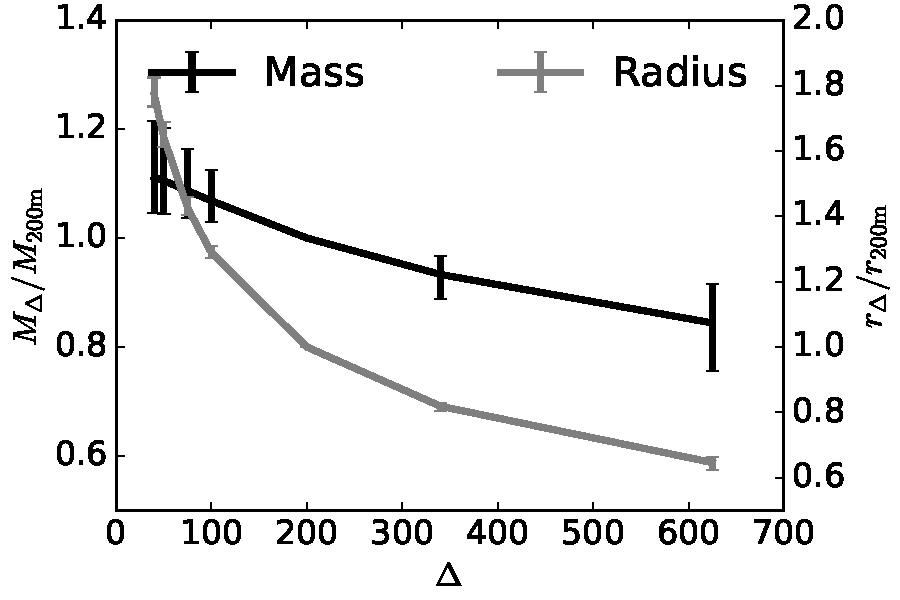
\includegraphics[width=\columnwidth]{massvsdelta_l0250.pdf}
\caption{
The ratio of halo properties as a function of $\Delta$ in the \simB~ catalog. The sample contains all host halos with masses greater than $M_{200\mathrm{m}} \ge 7.1 \times 10^{11}$. The black (dark grey) line shows the median value of the ratio of the halo mass (halo radius) at a value of $\Delta$ to the value at $\Delta=200\mathrm{m}$. The error bars contain 68\% of values of this ratio for the sample. 
\yao{this figure will be replaced by a $M_\Delta-\Delta$ plot}}
\label{fig:deltacompare}
\end{figure}

An additional benefit of the {\tt ROCKSTAR} software is the ability to identify substructure, commonly referred to in the literature as subhalos. All density peaks are identified within the simulation and if a halo exists within the phase space of another halo, the less massive of the two is defined to be a subhalo of the more massive companion. The more massive companion is referred to as the host halo. This process continues until all halos identified in the simulation have been designated as either host halos or subhalos.

%-------------------------------------
\section{Halo Properties}
\label{section:haloprops}
%-------------------------------------

As has long been well known, halo mass is the property that most strongly affects halo clustering. In 
this paper, we aim to study the strength of halo clustering as a function of halo properties other than 
mass. We will refer to these properties as ``auxiliary'' halo properties in this paper. Throughout the remainder of the paper, we refer to halo two-point clustering that depends upon one of these auxiliary properties at fixed mass variously as ``assembly bias,'' ``auxiliary property dependent'' clustering, or simply ``environmental dependence'' of the auxiliary property. The properties 
we study are described in this section.

%----------------------------------------
\subsection{Measures of Halo Concentration}

We investigate the clustering of halos as a function of a number of halo properties 
that have been shown to influence halo clustering at fixed halo mass. We explore 
two definitions of halo concentration. The first stems from a fit of the spherically-averaged 
halo density profile, $\rho(r)$, to a \citet{navarro_etal97} (hereafter, NFW) density profile, 
%
\beq
\rho(r) = \frac{\rho_0}{\frac{r}{r_{\mathrm{s}}}\left(1+\frac{r}{r_{\mathrm{s}}}\right)^2},
\eeq
%
\bdr{pedantic comment: the brackets in the above equation will look better if yuo use the right and left latex math commands.}where the density scale, $\rho_0$, and the scale radius, $r_{\mathrm{s}}$, are parameters 
that are fit to the density profile of each halo. The standard definition of halo concentration is then 
\beq
c_{\mathrm{NFW}} = \frac{\Rdel}{r_\mathrm{s}},
\eeq
where $\Rdel$ is the radius of the halo given an overdensity parameter, $\Delta$, defining the halo 
and $r_{\mathrm{s}}$ is the inferred halo scale radius. We use the NFW concentrations computed by the 
{\tt ROCKSTAR} halo finder, which are derived from a fit to the halo density profile.  


The NFW concentration defined in the previous paragraph has the shortcoming that it 
depends upon a parametric description of dark matter halos, so we study the clustering dependence 
of halos as a function of a non-parametric description of halo concentration as well. In particular, we 
use the ``velocity-ratio'' concentration,
\beq
c_{\mathrm{V}} = \frac{V_{\mathrm{max}}}{V_{\Delta}}, 
\eeq
where $V_{\mathrm{max}}$ is the maximum circular velocity achieved within the halo and $V_{\Delta}$ is 
the circular velocity at the halo radius, $\Rdel$. \bdr{Citations, e.g. Klypin's papers. I think they were the first to use this definition, but I'm not sure.}All halos of the same mass have the same value of $V_{\Delta}$; however, 
they exhibit a variety of $V_{\mathrm{max}}$ values depending upon the degree to which their masses are concentrated toward 
the halo centre. The quantity $c_{\mathrm{V}}$ is a non-parametric measure of halo concentration and can be measured from 
simulation snapshots without fitting halo density profiles. Consequently, $c_{\mathrm{V}}$ is robust to halo density 
profile parametrizations and halo profile fitting procedures. 


Halo concentrations are interesting to investigate for these purposes for a number of reasons. 
First of all, the environment dependence of halo concentrations is known to be strong for 
standard halo definitions. Second, halo concentrations are of interest in the modelling of 
galaxy clustering and gravitational lensing statistics (and their cross correlations). 
In the case of galaxy clustering, the relevance is indirect, because galaxies may 
not trace the mass densities of their host halos. In the case 
of gravitational lensing, the mass distribution is the primary quantity of interest and halo concentrations are 
directly related to predictions for lensing statistics. Third, concentrations can be measured from 
individual simulation snapshots easily and halo concentrations are known to be strongly correlated with 
the formation histories of dark matter halos with earlier forming halos having higher concentrations at 
fixed halo mass \citep{wechsler_etal02, zhao_etal03, wechsler_etal06, zhao_etal09}. 
As such, exploring the concentration dependence of halo
clustering may yield insight into the age dependence of halo clustering without the need for constructing merger
trees. \bdr{THe above paragraph could be shortened I think.}This is particularly important in the present study in which the halo finding is performed repeatedly for many 
different values of $\Delta$. Constructing a self-consistent merger tree from which halo formation history can be 
studied requires halo finding at all simulation snapshots for each new value of $\Delta$, which is a computationally 
prohibitive task. 

In the present paper, we limit our study to halo properties that can be measured from a single simulation 
snapshot. However, halo formation histories correlate with halo concentrations with significant scatter and this correlation may 
depend upon environment, so the reader should be wary of drawing conclusions about the environmental dependence of 
halo formation by extrapolating our results on halo concentration. 
We will explore measures of halo age directly in a forthcoming follow-up study dedicated to halo 
formation histories.

Figure~\ref{fig:cnfwrelation} shows the mean $c_{\mathrm{NFW}}$-$M_{\Delta}$ relation for halos defined with
$\Delta=200$ in \simA, \simB, and \simC. For each simulation, we consider halos only above a minimum mass threshold 
to ensure that property measurements are not compromised by resolution effects. The minimum mass 
thresholds are shown as the vertical lines in Fig.~\ref{fig:massrelation} and listed in Table~\ref{table:thresholds}. \bdr{What particle number do these thresholds correspond to?}
Figure~\ref{fig:massrelation} also shows the relation between the 
velocity-ratio concentration, $c_{\mathrm{V}}$, and halo mass. 
In the interest of completeness, Figure~\ref{fig:concentrations} shows the relationship 
between $c_{\mathrm{NFW}}$ and $c_{\mathrm{V}}$ on a halo-by-halo basis. As is evident, 
the two concentration proxies are strongly correlated and exhibit a $\sim 6\%$ scatter indicating 
that $c_{\mathrm{NFW}}$ and $c_{\mathrm{V}}$ indeed encode similar information about each 
halo.

%------------------------------------------ Figure for Cnfw(M)
\begin{figure*}
\centering
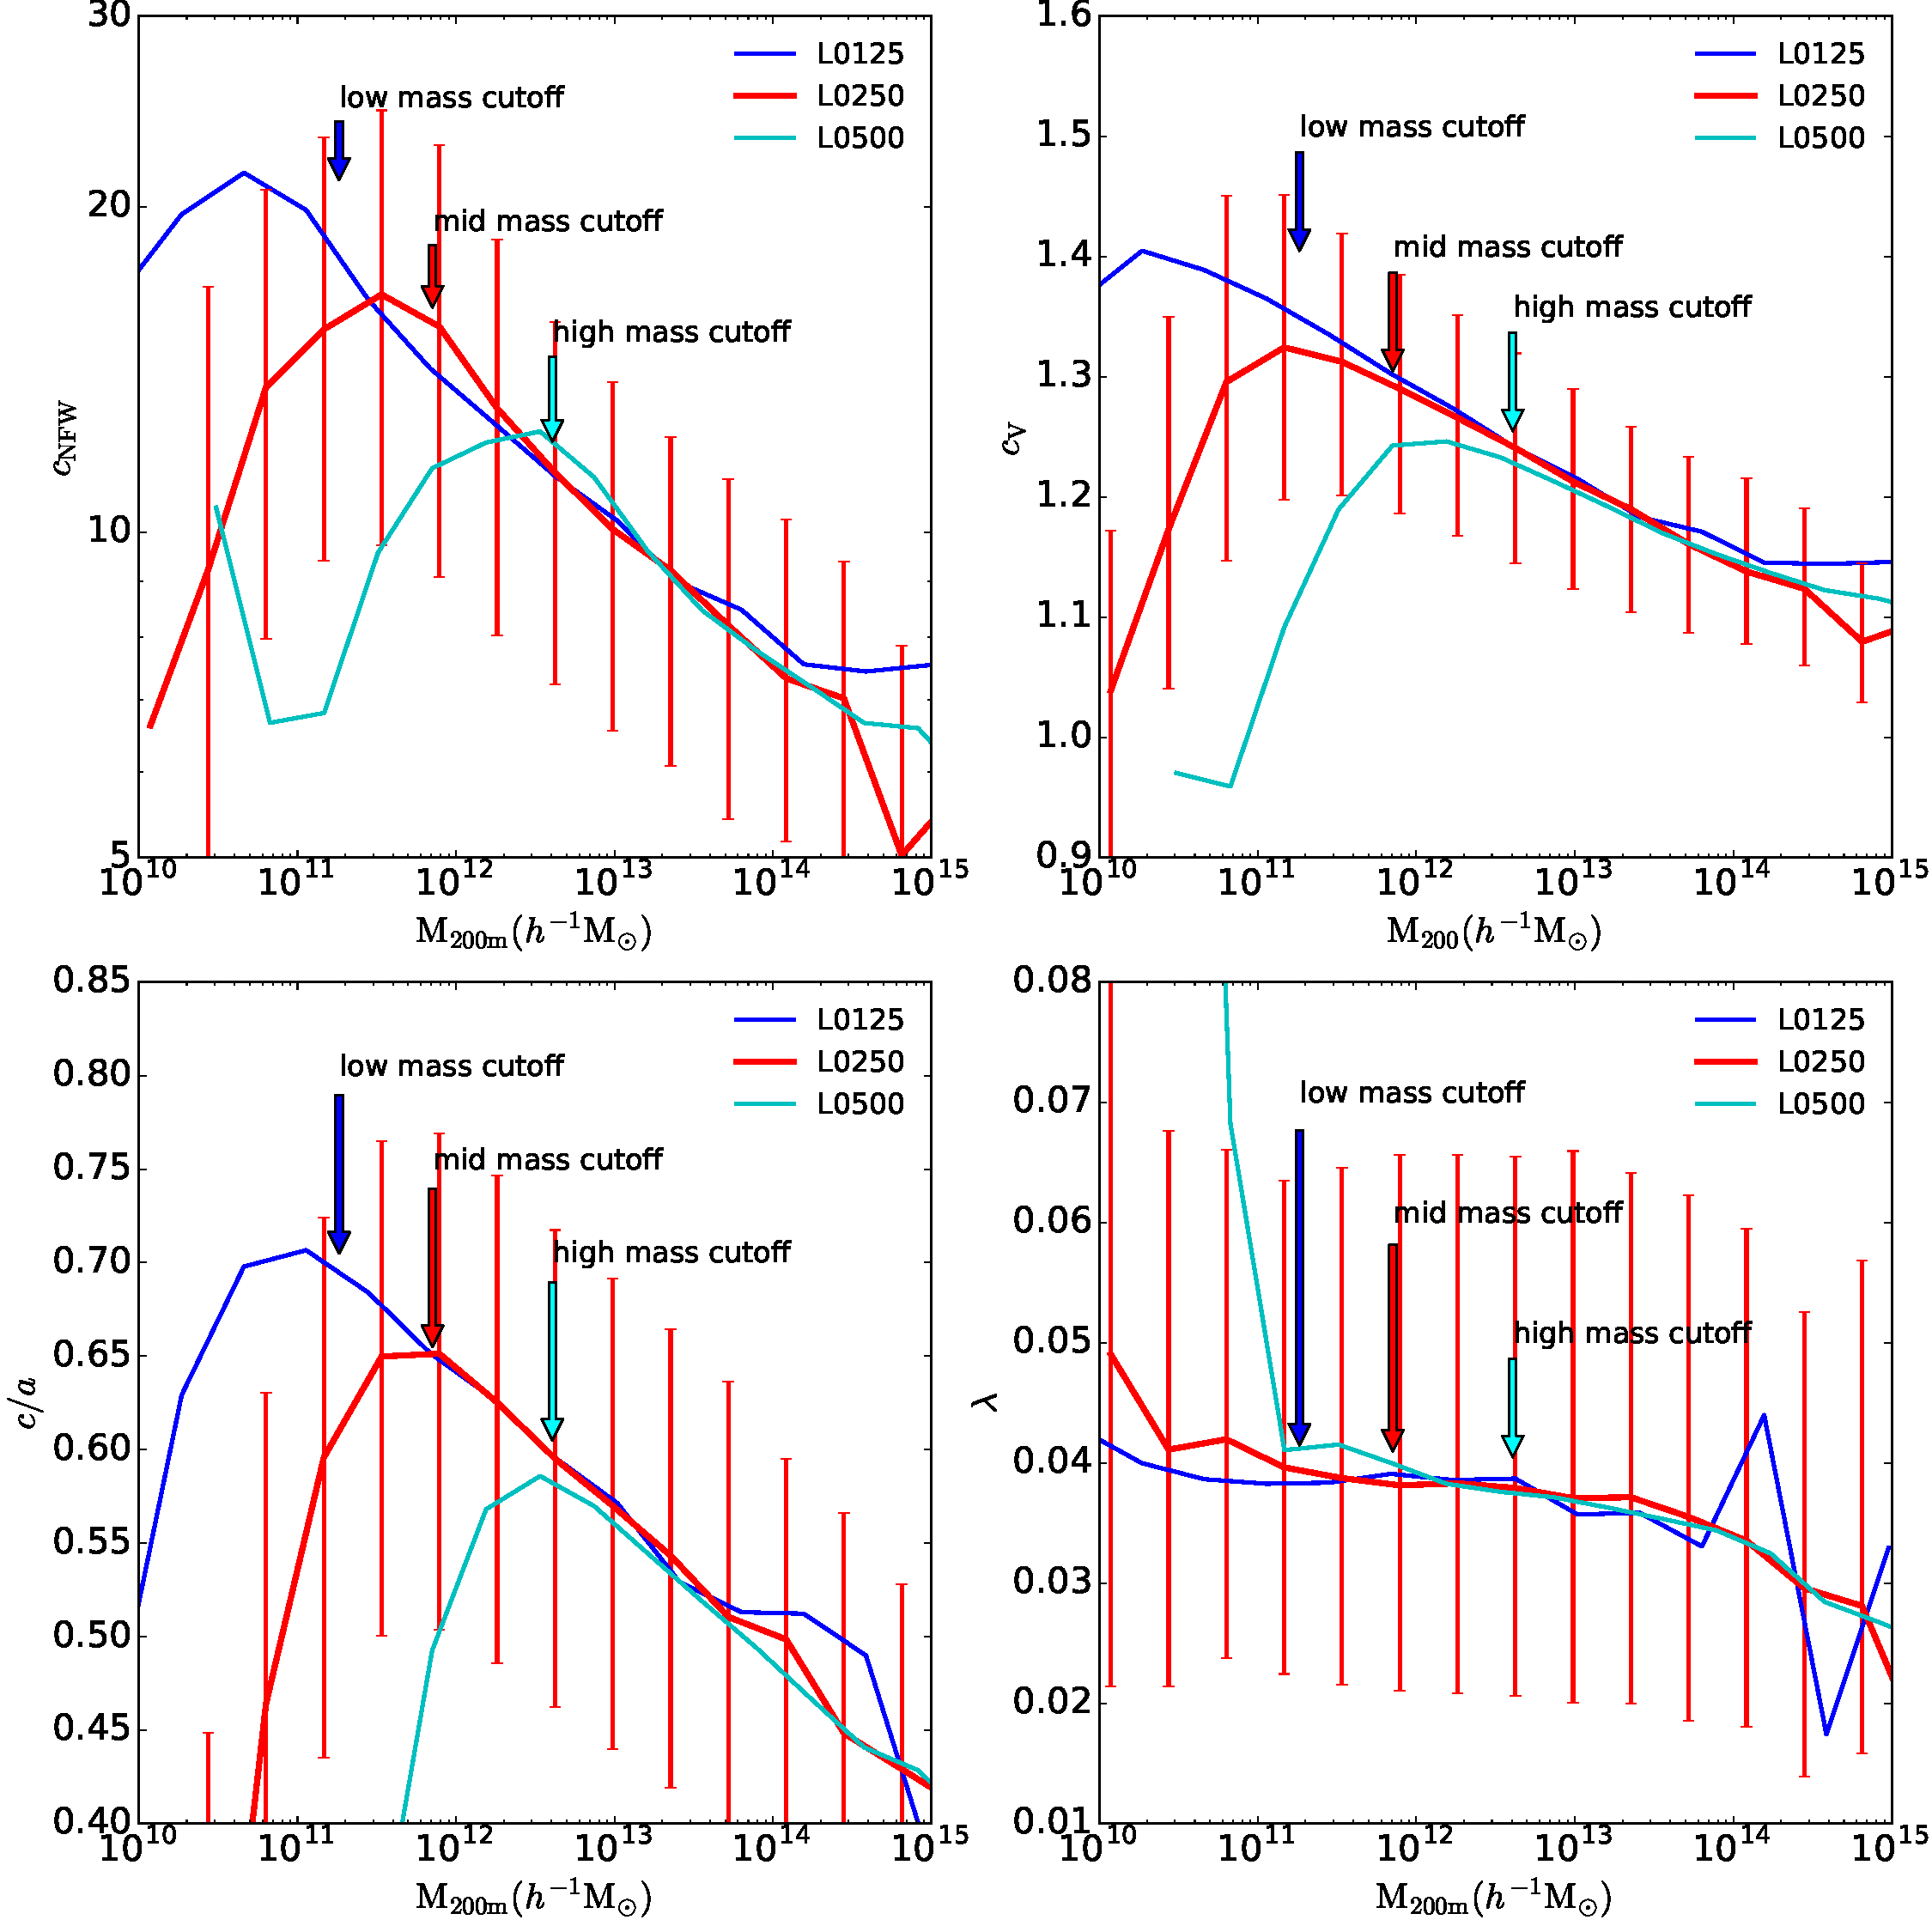
\includegraphics[width=\textwidth]{masscuts_d200.pdf}
\caption{
The relationship between halo properties and halo mass for each of our simulations with $\Delta =200$. These properties are the halo NFW-defined concentration, the velocity ratio defined concentration, the halo shape, and the halo spin.
In order of increasing simulation volume, the blue line corresponds to the concentration-mass relation from simulation 
\simA, the red line corresponds to \simB, and the cyan line corresponds to \simC. The red error bars show the 68\% spread in
parameter values within that mass bin for \simB. These errors are comparable to those of the other simulations
within the region of interest.
Each simulation is subject to resolution limitations at different halo masses. We show with arrows 
the minimum $M_{200}$ mass thresholds that we adopt in our analyses using the same colour code as 
the concentration-mass relations, going from \simA \ to \simC \ from left to right. Note the deviation from monotonic trends as a result of resolution effects.
\yao{Use a sequential colormap (same for Figures \ref{fig:cvrelation}, \ref{fig:srelation}, \ref{fig:spinrelation}). 
In fact, do we really need all four figures? But if so, can we consolidate them into a four-panel plots and reduce the repetition of caption text?}\asv{I had issues previously finding space for a readable 4-panel plot. I can give that a shot though.}
\bdr{I agree with Yao's comment: the four figures consume too much space and are confusing to the reader. Not sure what you mean by ``issues finding space''? The captions can be much compressed by combining the figures. The axis labels need to be much bigger on this figure. Finally, the error bars are OK but a shaded area would look more elegant.}\asv{Not sure I want to use a colormap given the different simulations rather than different $\Delta$, though can be changed quickly if needed.}
}

\label{fig:massrelation}
\end{figure*}
%--------------------------------------------------------------------------------



%-------------------------------------------- Figure comparing Cnfw and Cv on a halo-by-halo basis
\begin{figure}
\centering
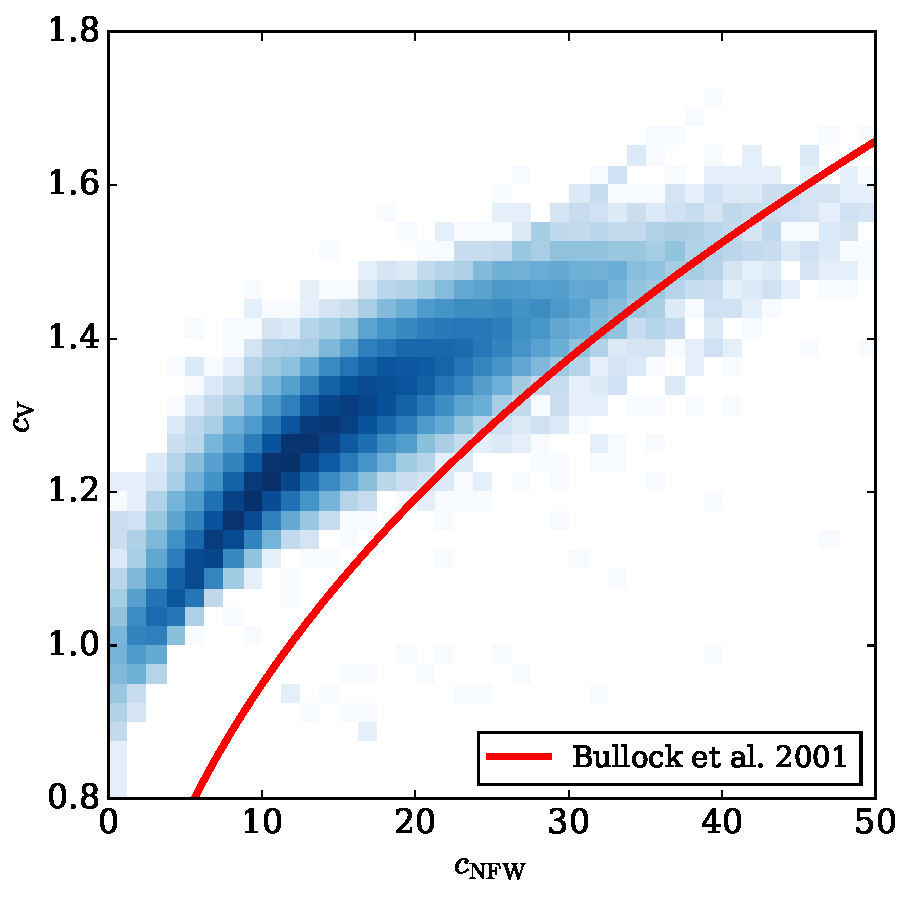
\includegraphics[width=\columnwidth]{cvvscnfw_relation.pdf}
\caption{
The relationship between the two different measures of concentration, 
using halos in \simB. The colour scale, shown at the right, encodes the number of halos 
within a single two-dimensional bin in the $c_{\mathrm{NFW}}$-$c_{\mathrm{V}}$ space. 
The red (blue) regions on the plot show where the most (fewest) halos exist with those values of the two
concentration parameters. The white regions indicate where no halos hold these values. The scatter on this relationship ranges from 5\% for intermediate concentration values, to a high of 13\% at high masses.
\yao{use a sequential colormap}
\bdr{When plotting 2D histograms, I think they always look better if the cells are square. The same goes for the overall plot - why should one axis be longer than the other?}}
\label{fig:concentrations}
\end{figure}
%--------------------------------------------------------------------------------------------------------------------------------


%---------------------------------------
\subsection{Halo Shape}

In addition to halo concentrations, we examine halo clustering as a function of a variety of other 
halo properties. We study halo clustering as a function of halo shape, $s$, 
quantified by the ratio of the halo minor, $c$ and major axis, $a$, lengths, 
%
\beq
s = \frac{c}{a}.
\eeq
%
The halo shapes we used were measured with {\tt ROCKSTAR} by calculating the mass distribution tensor,
\beq
M_{ij}=\frac{1}{N}\sum\limits_{N}\frac{x_i x_j}{r_{ij}^2},
\eeq
for
all particles within the halo radius, including particles associated with identified substructure, where $x_i$ is the position from the halo center along a given axis and $r_{ij}$ is the distance between the particle and the halo center and weights the overall calculation. The sorted eigenvalues of the matrix represent
the squares of the principal ellipsoid axes, where $a > b > c$. The mean relations for halo shapes as a function of halo mass for $\Delta=200$ are shown in Figure~\ref{fig:massrelation} along with the mass 
thresholds used to ensure that our results are not compromised by 
resolution.


%-----------------------------
\subsection{Halo Spin}

We study halo clustering as a function of halo angular momentum quantified 
by the spin parameter, $\lambda$, as introduced by \citep{peebles69},
\beq
\lambda = \frac{J \sqrt{\lvert E\rvert}}{G M_{\Delta}^{2.5}}
\eeq
where $J$ is the halo angular momentum, $E$ is the total energy of the 
halo, and $M_{\Delta}$ is the mass at the halo radius, $r_{\Delta}$. We measure this quantity using {\tt ROCKSTAR} which calculates the angular momentum, total energy, and total mass within $\Delta$ using bound particles out to the corresponding halo radius.
The mean relations for halo spin as a function of halo mass for $\Delta=200$ are shown in Figure~\ref{fig:massrelation} along with the mass thresholds enforced to ensure that our results are not compromised by resolution. These thresholds are summarized in Table~\ref{table:thresholds}, where we also show the threshold masses at various values of the overdensity parameter, $\Delta$.


%---------------------------------
\subsection{Halo Samples}

In practice, the mean relations between the various halo properties and the mass 
thresholds for our analyses must be determined separately for each combination of simulation, 
halo property (e.g., $c_{\mathrm{NFW}}$ or $s$), and halo definition (i.e., value of $\Delta$ in the case of the present study). 
For each analysis, we set mass thresholds in order to avoid the regime in which 
halo parameters are not well measured due to resolution limits of the simulations; 
we draw attention to the downturn in Figure~\ref{fig:massrelation} as an example of this, 
as the deviation from the underlying monotonic trend shifts to lower mass as we move from our lowest mass resolution to our highest mass resolution simulation, suggesting that this trend is driven by resolution alone.


For ease of comparison between halo definitions, we choose to use a single mass threshold for each
simulation and value of $\Delta$ whenever possible, rather than on a parameter-by-parameter basis. We summarize the mass thresholds we have used for a 
subset of $\Delta$ values in Table~\ref{table:thresholds}. 
At most values of $\Delta$, the minimum mass thresholds are 
driven by the requirement that the halo properties do 
not suffer significantly from finite resolution effects. We alert the reader to the fact 
that the mass of an individual halo will vary as $\Delta$ varies. This effect can be seen in Figure~\ref{fig:massmatch}, which demonstrates that while a decreased value of $\Delta$ leads to larger masses on average, there is a scatter due to changes in halo identification. Roughly speaking, 
the threshold masses in Table~\ref{table:thresholds} vary in such a way that the 
same physical objects are selected at each halo definition.

\bdr{General comment on section 3: it touches all the important points, but it could be shortened somewhat, in my opinion. After all, there is nothing genuinely new here, so I'd keep the language snappy and possibly even get rid of some equations that people have seen a million times (concentration...). Once again, a matter of taste of course.}






%%%%%%%%%%%%%%%%%%%%%%%%%%%%%%%%%%%%%%%%%%%%%%%%%%%%%%%%%%%%%%%%%%%%%%%%%%%%
\begin{table*}
\caption{
Minimum mass thresholds for each of our analyses. 
In the columns below each value of $\Delta$, we show the minimum 
host halo masses considered in units of $h^{-1}\mathrm{M}_{\odot}$.
Those rows without a label of ``-shape'' refer to the mass cut chosen for 
all analyses other than halo shape. Those rows with a label of ``-shape'' refer to 
the mass cut chosen for the shape parameter analyses. The latter require higher mass thresholds.\bdr{This may be personal taste, but to me this table would be much more useful in units of particle numbers. After all, resolution effects are due to poor resolution, not low halo mass.}}
\vspace*{8pt}
\begin{tabular}{ c c c c c c c }
\hline
\hline
Cutoff Name &  $\Delta=340$ & $\Delta=200$ & $\Delta=100$ & $\Delta=75$ & $\Delta=50$ & $\Delta=20$ \\
\hline
\vspace*{2pt}
{low mass} & $1.67 \times 10^{11}$ & $1.83 \times 10^{11}$ & $1.94 \times 10^{11}$ & $1.97 \times 10^{11}$ & $2 \times 10^{11}$ & $2.03 \times 10^{11}$  \\ \vspace*{4pt}
{mid mass} & $6.49 \times 10^{11}$ & $7.1 \times 10^{11}$ & $7.55 \times 10^{11}$ & $7.66 \times 10^{11}$ & $7.77 \times 10^{11}$ & {N/A} \\ \vspace*{4pt}
{high mass} & $3.71 \times 10^{12}$ & $4.06 \times 10^{12}$ & $4.31 \times 10^{12}$ & $4.38 \times 10^{12}$ & $4.44 \times 10^{12}$ & {N/A} \\
\hline \\
\end{tabular}
\label{table:thresholds}
\end{table*}
%%%%%%%%%%%%%%%%%%%%%%%%%%%%%%%%%%%%%%%%%%%%%%%%%%%%%%%%%%%%%%%%%%%%%%



%-----------------------
\section[]{Halo Clustering as a function of Auxiliary Halo Properties}
\label{section:methodology}
%-----------------------

%----------------------------------------------------------
\subsection{Auxiliary Halo Properties and Their Mass Dependence}
\label{subsection:properties}

We are interested in studying the clustering behavior of halos as a function of 
properties other than mass. As mass is the dominant halo property determining halo
clustering strength and environment, we refer to the other properties that we study as 
``auxiliary halo properties'' (those properties other than mass, such as concentration 
$c_{\rm NFW}$ or shape $s$). As has been demonstrated extensively in the literature, 
the auxiliary properties that we consider are themselves 
a function of mass \citep{bullock_etal02,allgood_etal06, duffy_etal08, despali_etal16}. 
This mass dependence, if not accounted for, induces clustering that depends upon these auxiliary properties in the absence of assembly bias. 
Most contemporary cosmological $N$-body simulations, and specifically the suite of simulations 
that we study in this work, do not have a sufficiently large number of halos to make isolating halos 
of fixed mass, and then further splitting these halos by an auxiliary property, a statistically 
powerful method with which to study the dependence of clustering on auxiliary properties. 
Therefore, it is necessary to remove and/or mitigate the mass dependence of the auxiliary 
properties that we study. 

We mitigate the mass dependence of the auxiliary properties as follows. First, 
we take all host halos more massive than our minimum mass thresholds and sort them by 
their halo masses, $M_{\Delta}$. We place these halos into twenty logarithmically-spaced bins 
of halo mass, ensuring that no bin has fewer than 10 halos\footnote{This is not true for the most massive bins which are limited to very rare objects. These have little statistical value and do not impact our results.}. 
We then calculate the rank of each auxiliary property within the bin of halo mass, from 1 to N, where N is the number of halos assigned to a given bin. If multiple halos share auxiliary property values (e.g. rank 2 and 3 have the same halo shape), then the average value of the rank is assigned to each halo (e.g. 2.5 to each). We normalize the rank distribution to be between 0 and 1 by dividing out the number of halos in the bin, resulting in a uniform distribution of ranks. This removes the strong mass trend in each of these properties. We use these normalized ranks of halo auxiliary properties to study halo clustering strength in the remainder of this work. We have experimented with different bin sizes and find that our qualitative results are not sensitive to the chosen number of bins. Furthermore, the choice of equally populated bins versus evenly spaced bins makes no significant difference to our results.

%---------------------------------------------------------------
\subsection{Clustering Statistics}
\label{subsection:clusteringstatistics}
%---------------------------------------------------------------


We assess the influence of assembly bias specifically on two-point statistics of host halos. In order to do so, we 
study both the standard two-point correlation functions of halos selected by properties other than mass 
(e.g., the auxiliary properties concentration, shape, and spin) as well as halo mark correlation functions
(MCFs). MCFs quantify the manner in which a halo property (the ``mark'') correlates among halo pairs as a function of the distance between the pairs. MCFs have the advantage that they effectively stack signal from all values of the halo auxiliary property, or mark, in contrast to selecting subsets of halos based on the auxiliary property. MCFs also stack signal from all environments and do not require any specific definition of halo environment in order to detect ``environmental'' trends that are usually referred to as assembly bias in the literature. Absent halo assembly bias, the halo marks are uncorrelated among pairs. 
MCFs have been used in many previous papers to quantify environmental dependence of halo 
properties other than mass \citep{sheth_tormen04,sheth05, harker_etal06,wechsler_etal06,mao_etal15}. 
Although it does not necessarily have to be the case, we find that using correlation functions of halo sub-samples and using MCFs lead to the same broad conclusions. 


For a specific halo property, or mark $m$, we use the MCF normalization of \citet{wechsler_etal06}, namely 
%
\beq
\mathcal{M}_m(r) \equiv \frac{\langle m_1 m_2 \rangle_p (r) - \langle m \rangle^2}{\mathcal{V}(m)},
\eeq
%
where $m_{\mathrm{i}}$ is the value of the mark for halo $\mathrm{i}$, $\langle m \rangle$ is the mean of the
mark, and $\mathcal{V}(m)$ the variance of the mark. The notation is intended to indicate that the average is
taken over all pairs of halos separated by a distance $r$. In the absence of any correlation between a halo
property among neighbors a separation $r$ away, $\mathcal{M}_m(r) = 0$. Deviations of the MCF from
zero indicate such correlations exist and the magnitude of $\mathcal{M}_m(r)$ gives the excess of the mark among
pairs compared to the one-point mean of the mark $\langle m\rangle$ in units of the one-point variance. The marks that we use are the normalized ranks of halo auxiliary properties described in Section~\ref{subsection:properties}. Therefore, these marks are distributed according 
to a uniform distribution from 0 to 1, such that $\langle m \rangle^2 = 0.25$ and $\mathcal{V}(m) = 1/12$. 


In each case, it is necessary to assess statistical fluctuations in the statistics that we measure in these simulations in order to determine the significance of the signals.\bdr{Phrasing: what is this sentence really saying?} For two-point correlation functions, we determine the covariance of the measurement through jackknife resampling of the eight octants of the simulation cube. 

We assess the significance of the MCFs by taking advantage of the inherent uniform distribution. For each halo we assign a random number drawn from a uniform distribution between 0 and 1. Since no information about the clustering was used in the assignment, the MCF calculated using this random number as this mark should trend to zero. We repeat this process 200 separate times and calculate the $2^{\mathrm{nd}}$ and $98^{\mathrm{th}}$ percentile values to determine the approximate 2 $\sigma$ interval. A signal within this range would be consistent with zero assembly bias. We note that since we investigate the product of two uniformly distributed variables, a negative value of the MCF has two different interpretations. One interpretation is that halos with enhanced (diminished) clustering correspond with higher (lower) values of the mark. The other possible interpretation is that more clustered halos tend to have a mixture of very high or very low mark values.\asv{Not quite sure how to phrase this - essentially, the second case you could imagine is if a host halo had very high concentration and was surrounded by other host halos with low concentration.} While we cannot distinguish between these two possibilities, it does not impact our ability to make statements about a potential non-detection of assembly bias, as our randomization implicitly accounts for the impact of a uniform product distribution.


%----------------------------
\section[]{Results}
\label{section:results}
%----------------------------


%-----------------------------------------------
\subsection{Correlation Functions}
\label{sub:cfresults}


We begin by studying the correlation functions of halos in our mass threshold samples, sub-selected by auxiliary
properties. Figure~\ref{fig:cc_cfcompare} exhibits the difference between the clustering strength of halos in the
$20^{\mathrm{th}}$ percentile highest NFW concentrations and the halos with the halos that have the
$20^{\mathrm{th}}$ percentile lowest NFW concentrations as a function of the overdensity parameter, $\Delta$, used to
define the halos. In order to make the differences more apparent, the two-point functions in 
Fig.~\ref{fig:cc_cfcompare} have been normalized by the clustering strength of the entire halo sample. 


If the clustering strength of halos were independent of halo concentration, we 
would expect the lines in Fig.~\ref{fig:cc_cfcompare} to cluster around zero (scattered about zero by finite sample size). 
The evident deviations demonstrate that halos of different NFW concentrations exhibit appreciably 
different clustering, a fact that is already well known and has been studied by a number of authors. 
Furthermore, it is clear that the strength and sign of assembly bias due to NFW concentration is 
strongly mass dependent for any fixed halo definition, a result that also agrees with the significant 
previous literature on halo assembly bias using conventional halo definitions 
\citep{wechsler_etal02, gao_etal05, zentner07, wechsler_etal06, harker_etal06, croton_etal07, dalal_etal08, mao_etal15, sunayama_etal16}.
At relatively low mass (the low-mass panel, $M_{200} > 1.83 \times 10^{11} \hMsun$), 
high-concentration halos are considerably more strongly clustered than low-concentration halos using the more 
conventional $\Delta = 200$ definition for halos. At somewhat higher halo masses 
(e.g., the mid-mass panel, $M_{200} > 7.1 \times 10^{11} \hMsun$), this difference is markedly reduced. 
Finally, for the highest-mass halos that we have the capability of studying (the high-mass panel, 
$M_{200} > 4.06 \times 10^{12} \hMsun$), the effect is weaker and also of opposite sign; 
low-concentration halos are more strongly clustered than high-concentration halos.

Focus, for example, on the middle panel of Fig.~\ref{fig:cc_cfcompare}. In this panel, 
corresponding to the mid-mass threshold, the difference in large-scale clustering between 
high- and low-concentration halos is dramatically reduced for a halo definition with 
$\Delta \approx 40$ as compared to a more traditional halo definition, such as $\Delta=200$. 
However, further decreasing $\Delta$ leads to concentration-dependent clustering of opposite sign. 
Both the strength and the sense of halo assembly bias depend upon halo definition! This is a 
point that may seem somewhat obvious in retrospect, but does not seem to be addressed 
explicitly anywhere in the literature despite its importance.


Comparing the differing clustering strengths across the three panels of Fig.~\ref{fig:cc_cfcompare}, 
it is clear that any specific conclusions about concentration-dependent halo clustering 
vary with halo mass. For low-mass halos (the top panel), 
very low values of $\Delta$ (and correspondingly large definitions of halo radii, 
as $R_{\Delta}$ very roughly in proportion to $\Delta^{-1/3}$) are necessary in order 
to mitigate the concentration dependence of halo clustering. Conversely, for higher-mass 
halos (the bottom panel), conventional values of $\Delta \sim 200-340$ yield little 
concentration-dependent clustering. In this case, decreasing $\Delta$ (increasing $R_{\Delta}$) 
results in significantly {\em increased} concentration dependent halo clustering. The reasons for 
these changes are of interest and we return to the interpretation of these results below.


Notice that in all panels of Fig.~\ref{fig:cc_cfcompare}, the effect of concentration-dependent clustering is
mildly scale-dependent. Moreover, this scale dependence is evident for all values of $\Delta$. Simply
defining halos with a different value of $\Delta$ does not suffice to eliminate concentration-dependent
clustering on all scales. In this discussion and throughout, we focus primarily on the large scale clustering,
which we take to mean clustering on scales significantly larger than the radii, $R_{\Delta}$ of the halos in our
samples.


%---------------------------------------------------------------------------------------------------------------------------------------
\begin{figure*}
	\centering
	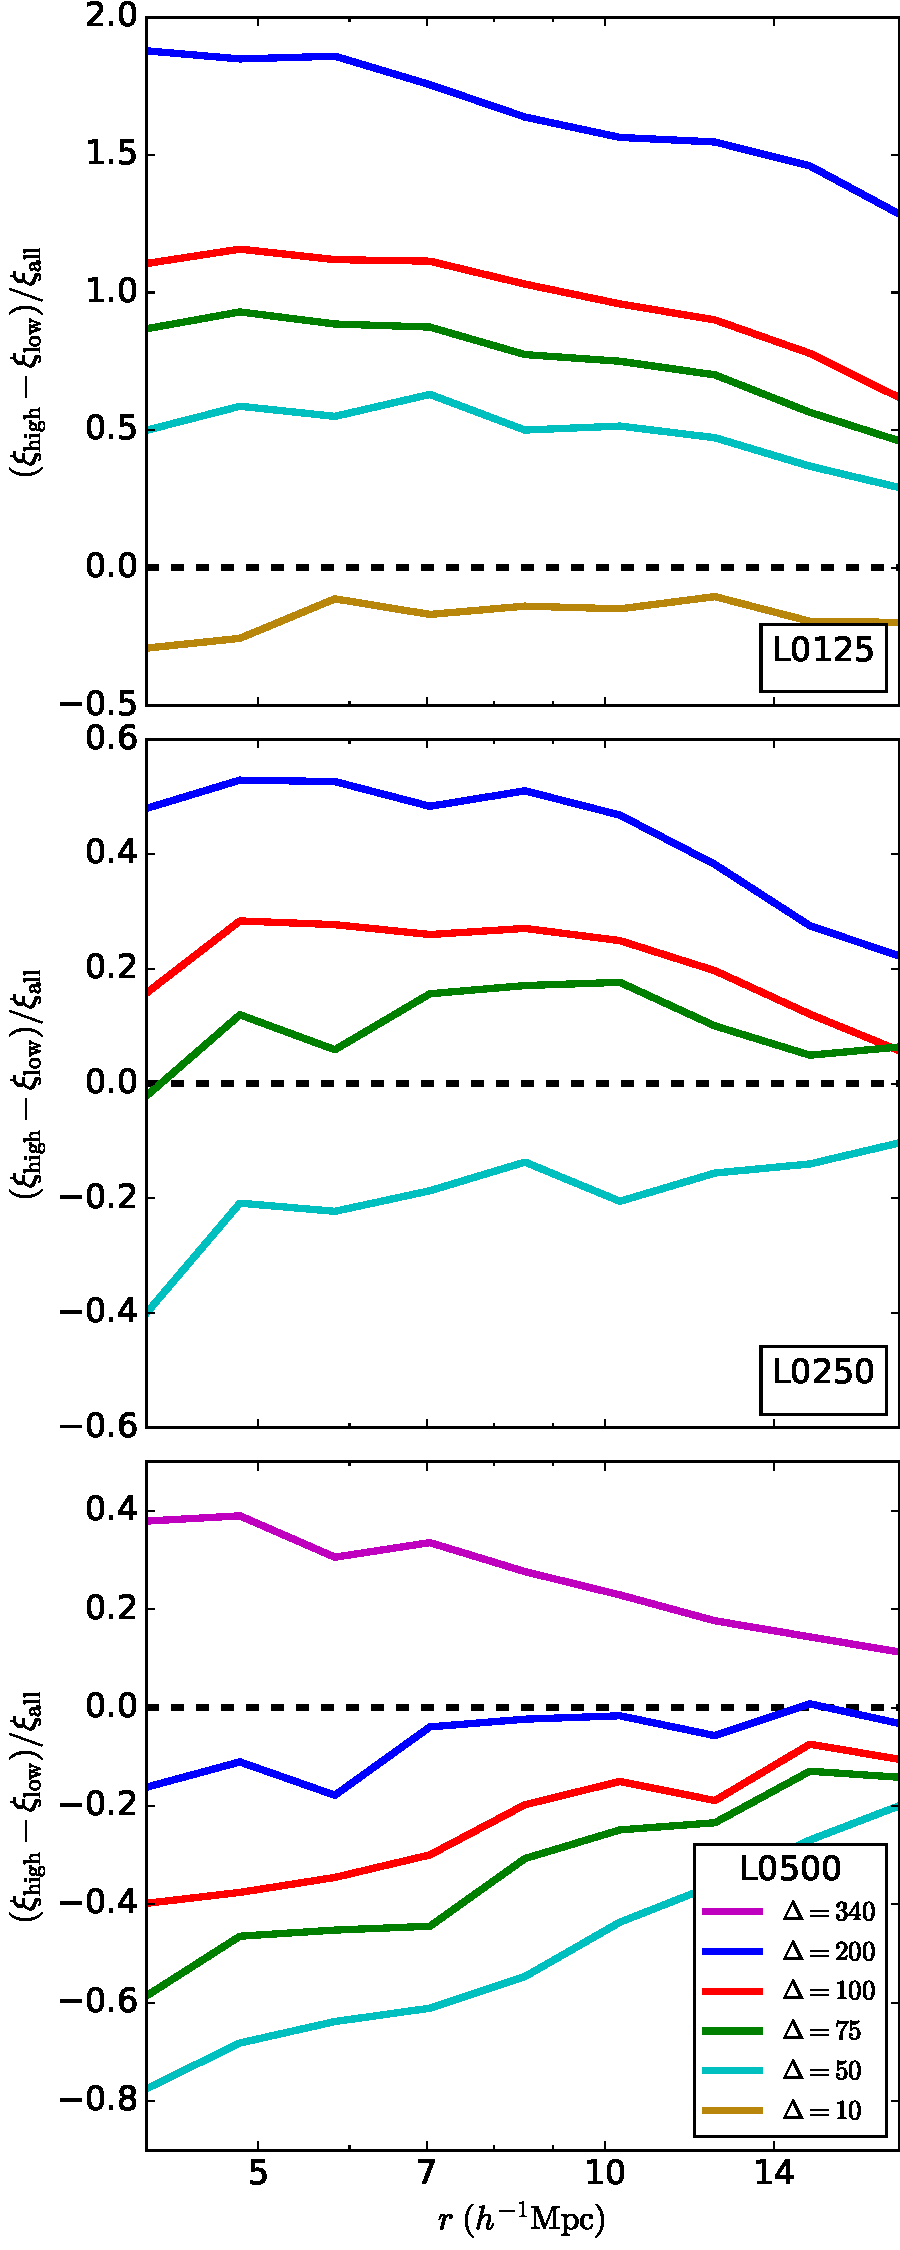
\includegraphics[width=\textwidth]{all_cfcompare_cnfw.pdf}
	\caption{
In each panel, the solid lines plot the difference between the correlation function for the top
20\% and the bottom 20\% of halos by NFW concentration, normalized by the
correlation function of the entire sample. In each plot the lines correspond to different values of $\Delta$, with dark blue (light blue) corresponding to $\Delta = 340$ ($\Delta = 50$). The 
 line corresponds to the overdensity chosen for matching as possibly removing assembly bias on most scales in the case of halo concentration.
The top (middle/bottom) panel shows the results for the \simA \ (\simB /\simC) data 
set utilizing the low mass (mid mass/high mass) cutoffs. Error bars correspond to the two $\sigma$ error on the measurement.\bdr{The legends are a little confusing. When I look at the main legend in the bottom panel, I thought that the red dashed line was Delta = 200 in all panels, because the little legends in those panels are very small. I'd separate the legends also in the bottom panels and make the red-line legend much bigger to highlight that those lines represet different Deltas.}
}
\label{fig:cc_cfcompare}
\end{figure*}
%----------------------------------------------------------------------------------------------------------------------------------------------


It should be noted that this method is robust to the choice of samples. For instance, 
changing from examining the $20^{\mathrm{th}}$ percentile of concentrations to another 
value (e.g., $10^{\mathrm{th}}$ or $50^{\mathrm{th}}$ percentile) 
does not change the conclusions drawn from Fig.~\ref{fig:cc_cfcompare} significantly. In the 
case of halo concentration, adopting $c_{\mathrm{V}}$ rather than $c_{\mathrm{NFW}}$ 
also does not alter our conclusions. Therefore, we do not show these additional results 
in the interest of brevity.

Furthermore, we note that quite generally, for each of the halo properties we have studied, 
the conclusions drawn from examining correlation functions are the same as those drawn from 
studying MCFs. Consequently, we now move on to a more comprehensive 
discussion of the strength of auxiliary property-dependent halo clustering using MCFs. 

\bdr{General comment on Figures 8-14: they look good overall, clear and not too crowded. However, they do take up a lot of space, and having so many figures might look a bit scary to some readers. One solution that I could see which would not take a lot of effort would be to re-arrange the panels so that each property occupies a row rather than a column, sharing the y-axis. This would make it easier to quantify the mass dependent normalizations of the lines which is a little difficult right now. In this arrangement, multiple properties could be ``stacked'' into one figure to save space and caption text. For example, the first figure could be the current figure 8 (correlation function), the second one figures 9-10 (concentrations) and the third figure 11-12 (shape / spin, with a caption just saying ``same as figure X, but...''.}

%-----------------------------------------------------------------
\subsection{Mark Correlation Functions}
\label{sub:mcfresults}

\begin{figure*}
	\centering
	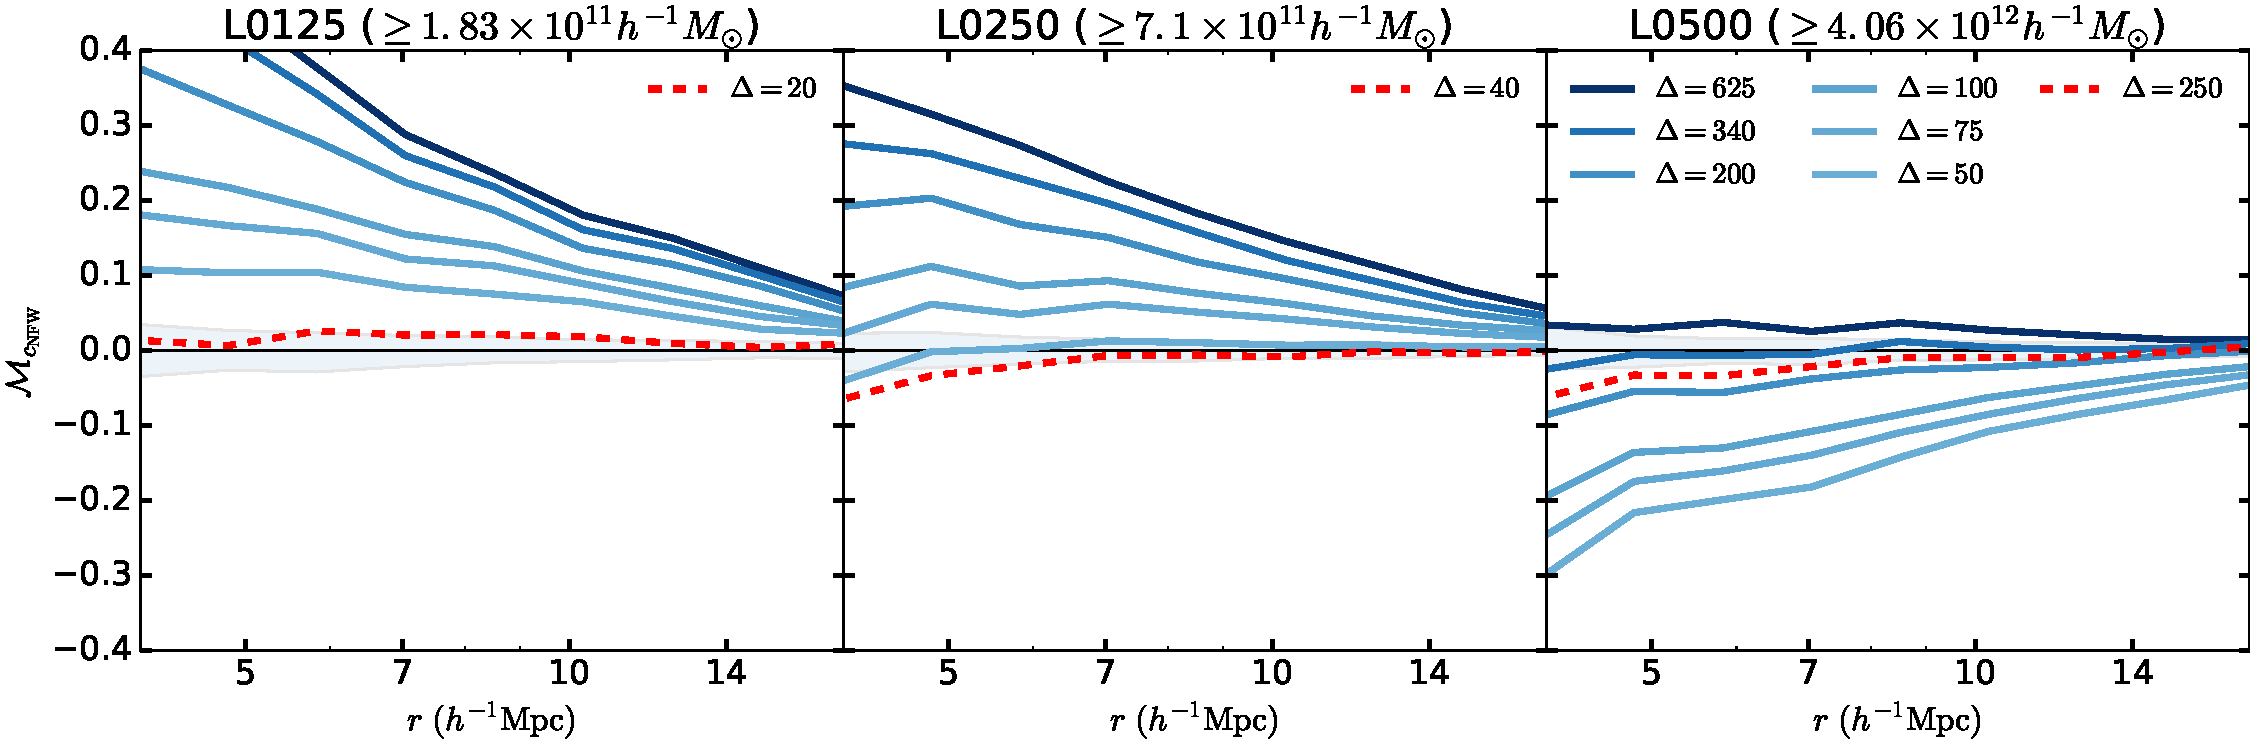
\includegraphics[width=\textwidth]{all_mcf_cNFW.pdf}
	\caption{
The marked correlation function for the concentration defined according to the NFW profile. The solid lines plot the marked correlation function using normalized ranks of NFW concentration as the mark. In each plot the lines correspond to different values of $\Delta$, with dark blue (light blue) corresponding to $\Delta = 340$ ($\Delta = 50$). The red dashed line corresponds to the overdensity chosen for matching as possibly removing assembly bias on most scales in the case of halo concentration. The top (middle/bottom) panel shows the results for the\simA \ (\simB /\simC) data set utilizing the low mass (mid mass/high mass) cutoffs. The shaded bands represent 2-sigma confidence regions generated by randomization of the marks.
}
	\label{fig:cc_mcf_cnfw}
\end{figure*}


%------------------------
\subsubsection{Halo Concentration}

The NFW concentration, $c_{\mathrm{NFW}}$, MCF is shown in Figure~\ref{fig:cc_mcf_cnfw}. 
The shaded bands in the figure delineate the statistical fluctuations in MCFs induced by 
finite sampling as discussed in Section~\ref{subsection:clusteringstatistics}. 
Qualitatively, Fig.~\ref{fig:cc_mcf_cnfw} exhibits the same features that are evident in 
Fig.~\ref{fig:cc_cfcompare}: more concentrated halos are significantly more clustered in 
the low-mass cut L0125 halo sample; concentration-dependent halo clustering weakens and 
reverses sense as halo mass increases (at fixed $\Delta$), 
consistent with work on assembly bias \citep{wechsler_etal06,sunayama_etal16}; for the 
mid-mass cut L0250 sample with $\Delta=40$, the large-scale concentration dependence of halo clustering has been reduced so as to 
be consistent with zero within the statistical limitations of the simulation. 

Figure~\ref{fig:cc_mcf_cV} is a similar plot for the MCF of the velocity-ratio concentration, $c_{\mathrm{V}}$. 
This figure exhibits qualitatively very similar features to Fig.~\ref{fig:cc_mcf_cnfw}, a 
fact that is not surprising given that we already know that $c_{\mathrm{NFW}}$ and $c_{\mathrm{V}}$ 
quantify largely redundant information about their halos.

%---------------------------------------------------
\begin{figure*}
	\centering
	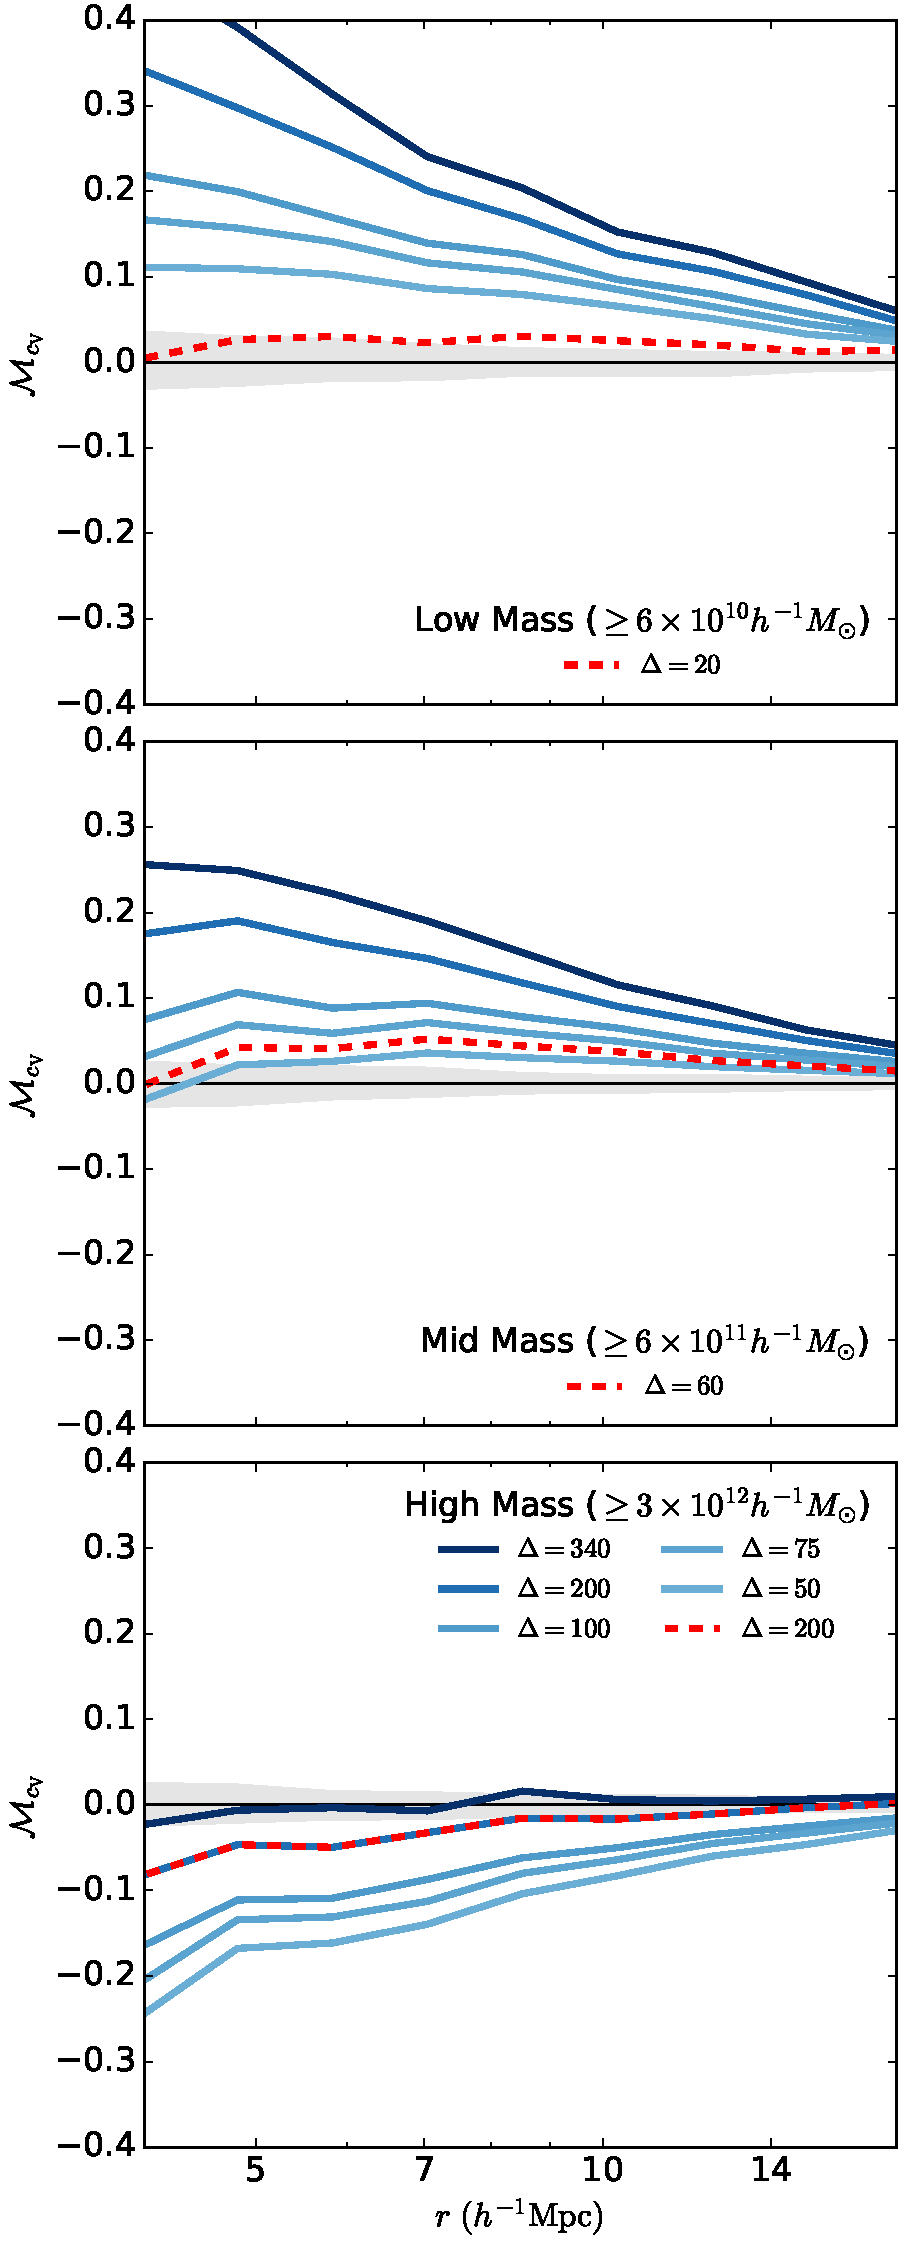
\includegraphics[width=\textwidth]{all_mcf_cV.pdf}
	\caption{	
As Fig.~\ref{fig:cc_mcf_cnfw}, with the mark being defined as the velocity ratio defined halo concentration.
\yao{This figure is almost identical to Fig.~\ref{fig:cc_mcf_cnfw}. Do we really need both? The rank correlation coefficient between $c_V$ and $c_{\rm NFW}$ must be high and one would expect this result.}\asv{Definitely true, but I think the value to having both is that it is suggestive that this is independent of how you define the halo density profile. If we think this is too much, we could certainly cut $c_{\rm NFW}$.}
}
	\label{fig:cc_mcf_cV}
\end{figure*}
%---------------------------------------------------


%----------------------
\subsubsection{Halo Shape}

%--------------------------------------------------- Shape MCFs
\begin{figure*}
	\centering
	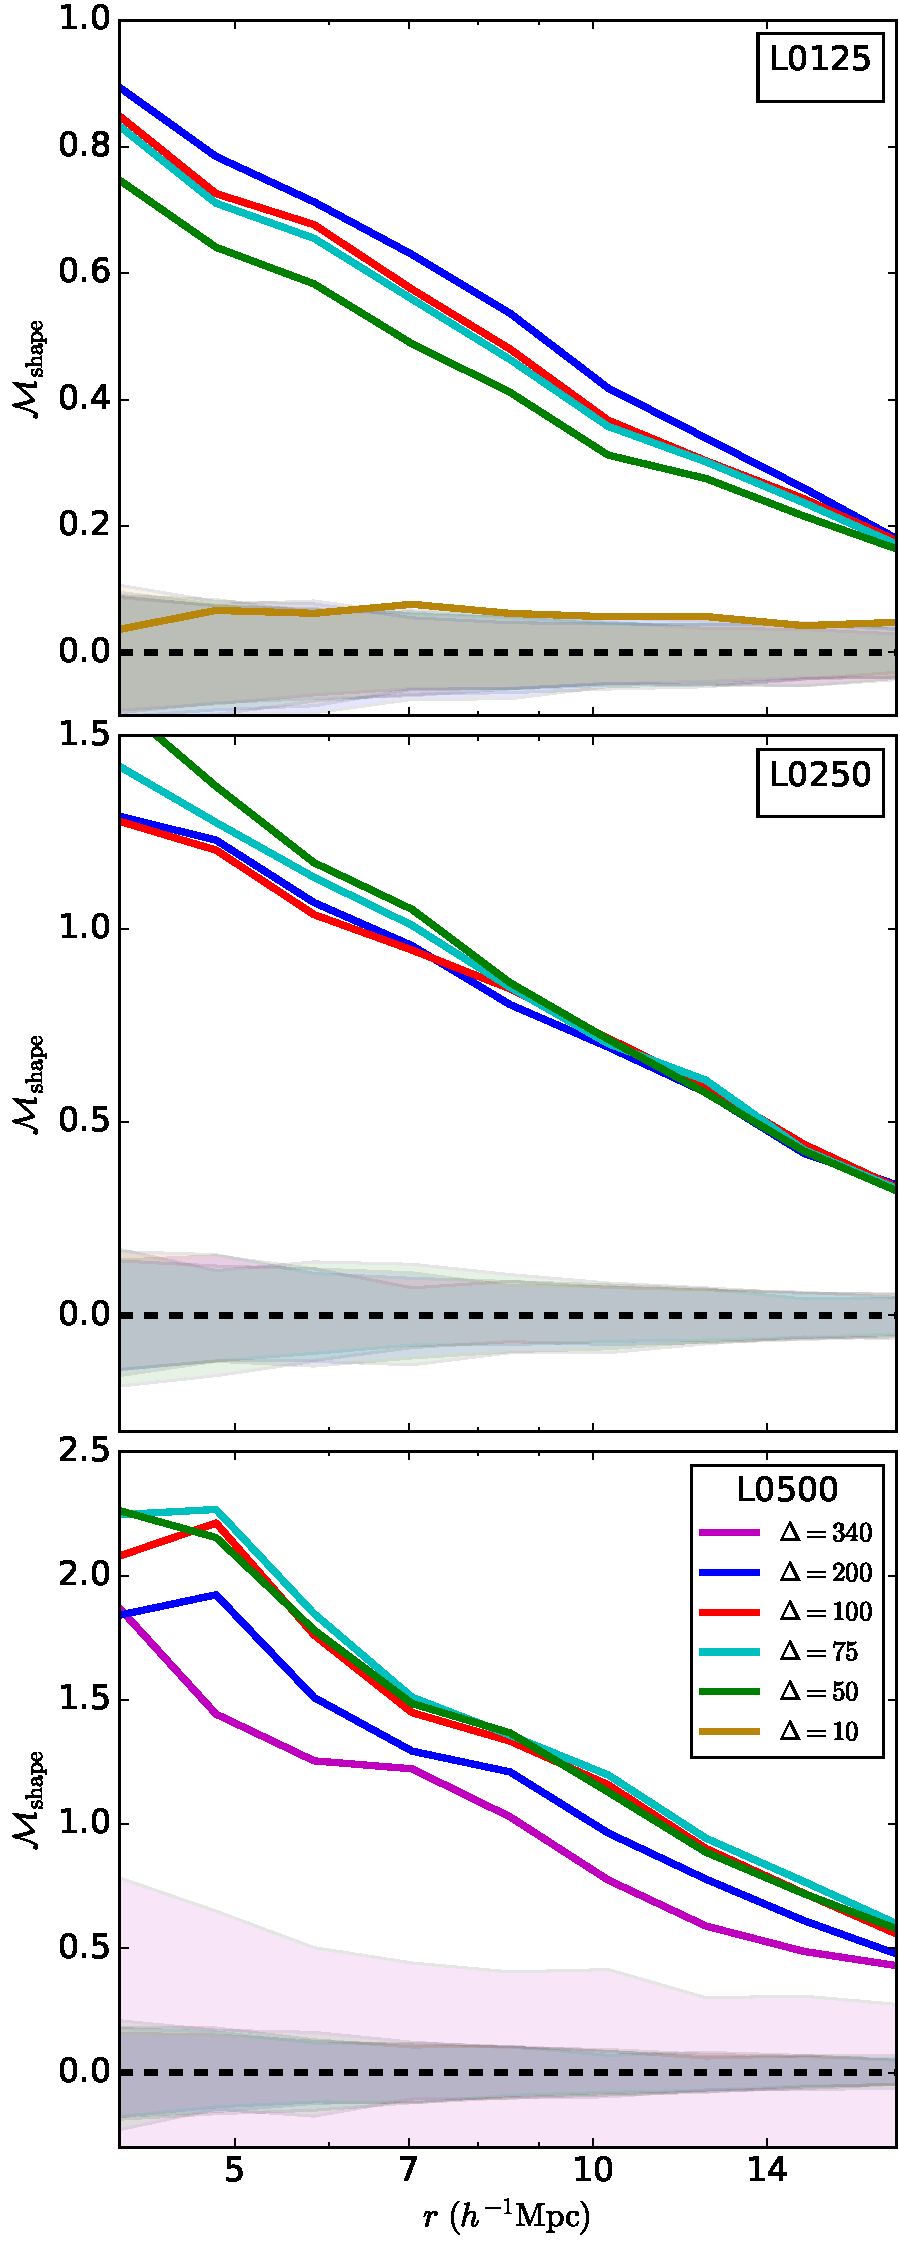
\includegraphics[width=\textwidth]{all_mcf_shape.pdf}
	\caption{
As Fig.~\ref{fig:cc_mcf_cnfw}, with the mark being defined as the halo shape.
\yao{This is likely to be too much work, but I think it would be more concise if you can summarize Fig.~\ref{fig:cc_mcf_s}, \ref{fig:cc_mcf_spin}, \ref{fig:cc_mcf_nsat} into plots like Fig.~\ref{fig:biascompare}. }\asv{They actually show slightly different things - Fig.~\ref{fig:biascompare} uses a limited subset of the masses which results in a noisier measurement, whereas this has a single lower mass threshold. I think there is definite value to both.}}
	\label{fig:cc_mcf_s}
\end{figure*}
%--------------------------------------------

\arz{A few comments here on the shape disussion and on Figure~\ref{fig:cc_mcf_s}. First, does your discussion really 
go with what is shown in the plot? I see that going down to 
$\Delta=20$ helps A LOT. Related to this, the red dashed lines 
in the middle and bottom panels don't make sense? They are clearly 
not the best case scenarios. In fact, it looks to me like the best 
case should be $\Delta=20$ in ALL PANELS! Am I missing something? Finally, you don't discuss Figure~11 AT ALL in the paper? Is it necesssary? I think probably not?}
\asv{Added in lines about how our red dashed lines are best case with regards to halo concentration. I also will remove the figure on how shape evolves with $\Delta$ - that was more relevant when we were getting shape measurements that were anomalous with previous paper results.}
Moving on from concentrations, Figure~\ref{fig:cc_mcf_s} illustrates MCFs in which the mark is the normalized rank of the shape parameter, $s$, of the halo. Similar trends as the previous cases repeat themselves in the case where shape is used at the trace mark. For the entire range of halo masses studied, the fiducial halo definition shows that more clustered halos have more spherical halos (e.g. halos with larger $s$ values). Furthermore, our change in halo definition shows that increasing the size of halos (and decreasing $\Delta$) leads to the most clustered halos having less spherical halos. Note that the shape-driven assembly bias appears to have minimal dependence on halo mass.

Where the environmental dependence associated with the shape parameter distinguishes itself is in finding the best fit value of $\Delta$ for removing the halo assembly bias. No reasonable value of $\Delta$ seems to be
capable of removing the enhanced clustering at the scales that we study, though the impact is reduced. We note that the best fit matches for concentration, the red-dashed lines in Figure~\ref{fig:cc_mcf_s}, do not correspond with removing assembly bias from shape. This failure may be driven by the filamentary nature of large-scale structure. Halos in overdense regions will gain mass as their halo radius expands that is not associated as substructure. If this additional mass accumulates with a preferred direction, as may be expected along a filament, this could induce a more elliptical halo shape. A detailed test of this hypothesis is beyond the scope of this paper, but may well be testable through association of halos with large-scale structure.

%---------------- spin MCF
\begin{figure*}
	\centering
	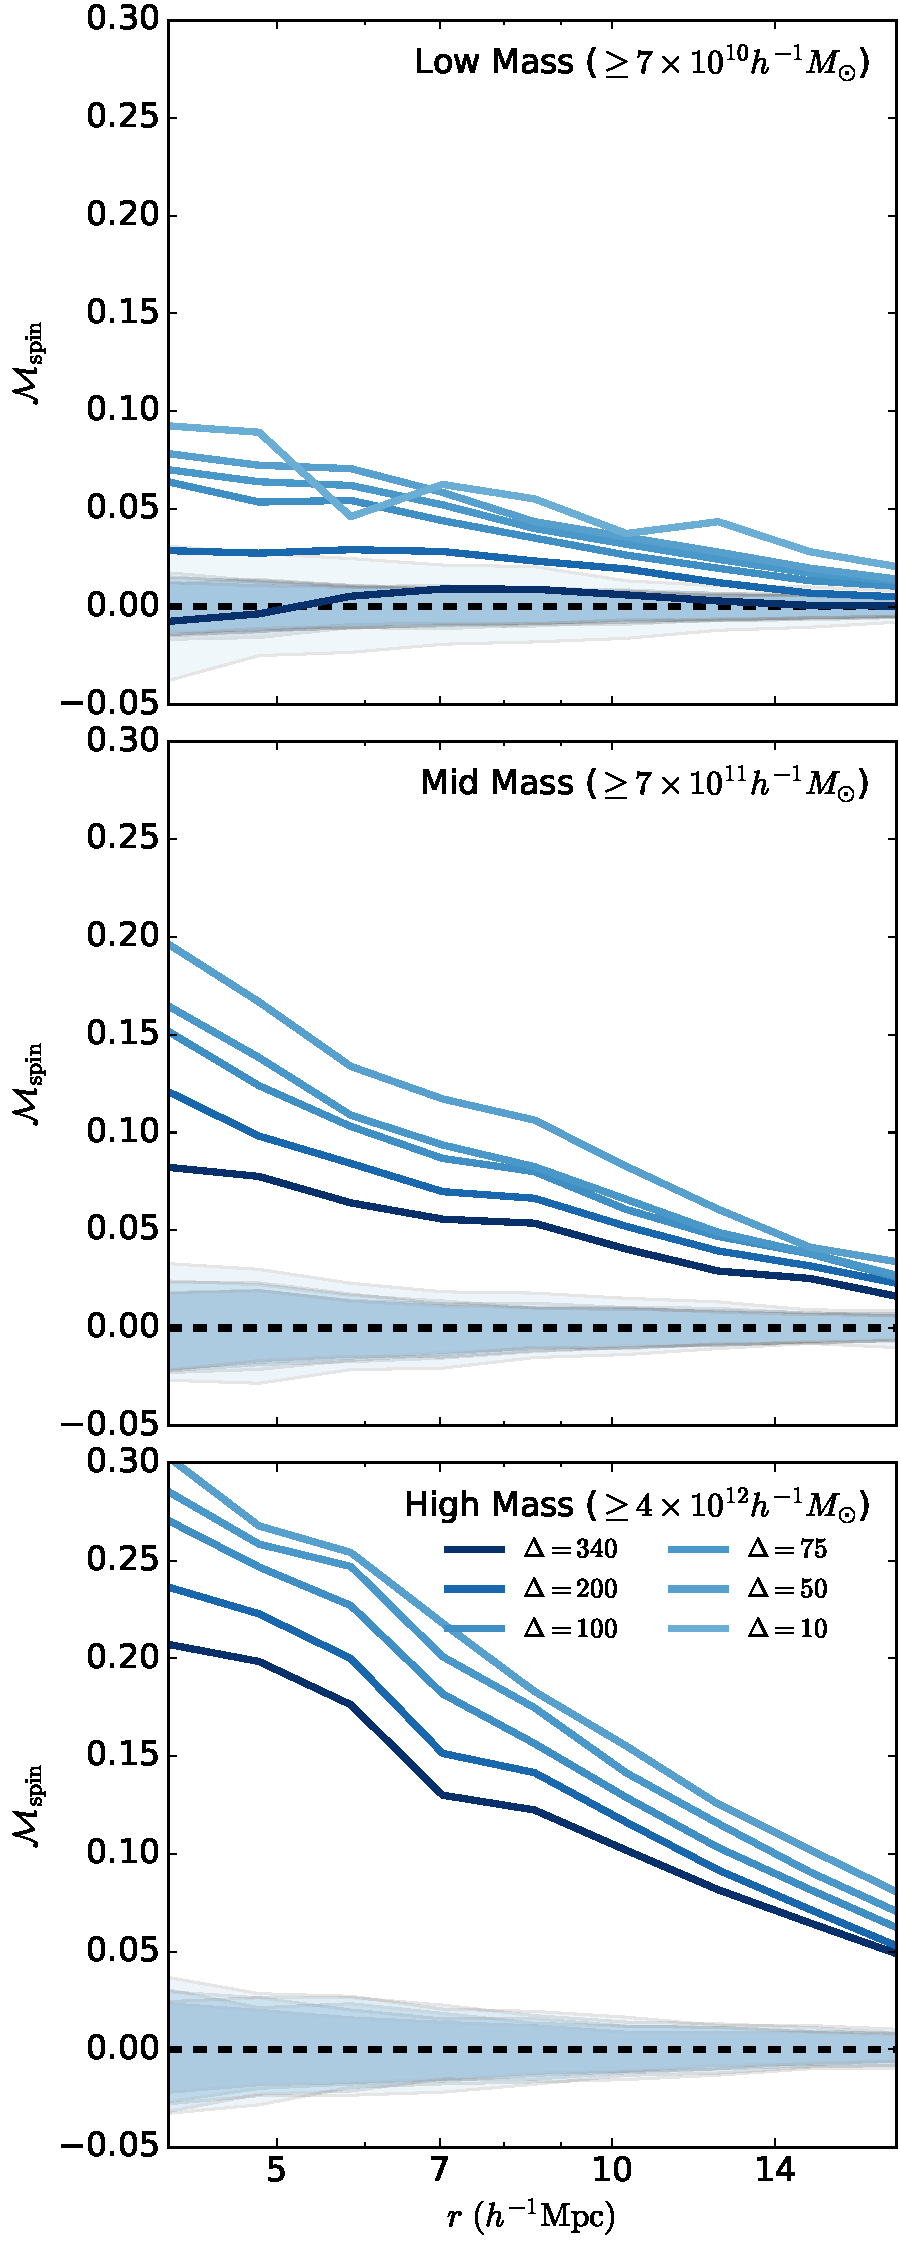
\includegraphics[width=\textwidth]{all_mcf_spin.pdf}
	\caption{
As Fig.~\ref{fig:cc_mcf_cnfw}, with the mark defined as halo spin.
\yao{see my comment on Fig.~\ref{fig:cc_mcf_s}}}
	\label{fig:cc_mcf_spin}
\end{figure*}
%-------------------------------

%------------------
\subsubsection{Halo Spin}

The spin MCFs are shown in Figure~\ref{fig:cc_mcf_spin}. Halos that are more clustered show higher values of the spin mark than would be expected from a uniform distribution of ranks, consistent with results in the literature \citep{bett_etal07,faltenbacher_white10,lacerna_padilla12}. Further, halos of higher mass show stronger spin-driven assembly bias; for the least massive halos ($M_{200} > 1.83 \times10^{11}\hMsun$) we see that $\Delta=340$ has minimal assembly bias, while higher mass bins would demand significantly higher $\Delta$. As with halo shape, it can be seen that the best matches for halo concentration (the red-dashed lines in Figure~\ref{fig:cc_mcf_spin}) are poor fits for removing assembly bias from halo spin.\arz{Search the literature, particularly Brandon Allgood's papers and Andreas Faltenbacher whose 
names come to mind, for spin-dependent assembly bias. I'm trying to figure out if yours is the first paper 
to point this out.}\asv{Need to track down all the specific citations, but after changing our normalization
method, it seems to match up better with existing texts.}
\arz{Citations here still need to be done.}\asv{Can't find the Allgood citation for spin as first author. I'll do another pass.} However, halo spin shows a qualitative response to our methodology opposite from that of halo concentration or halo shape. Increasing halo radii by decreasing $\Delta$ only serves to increase the impact of assembly bias in this case; effectively our newly defined halos have higher spins than average in this case. As with halo shape, one can invoke a model relating back to filamentary structure. If new material is accumulated along some preferred direction, it is not unreasonable to conclude an increased value of spin. This might enhance the impact of assembly bias as a result of our method.



%----------- NFW match figure
\begin{figure*}
	\centering
	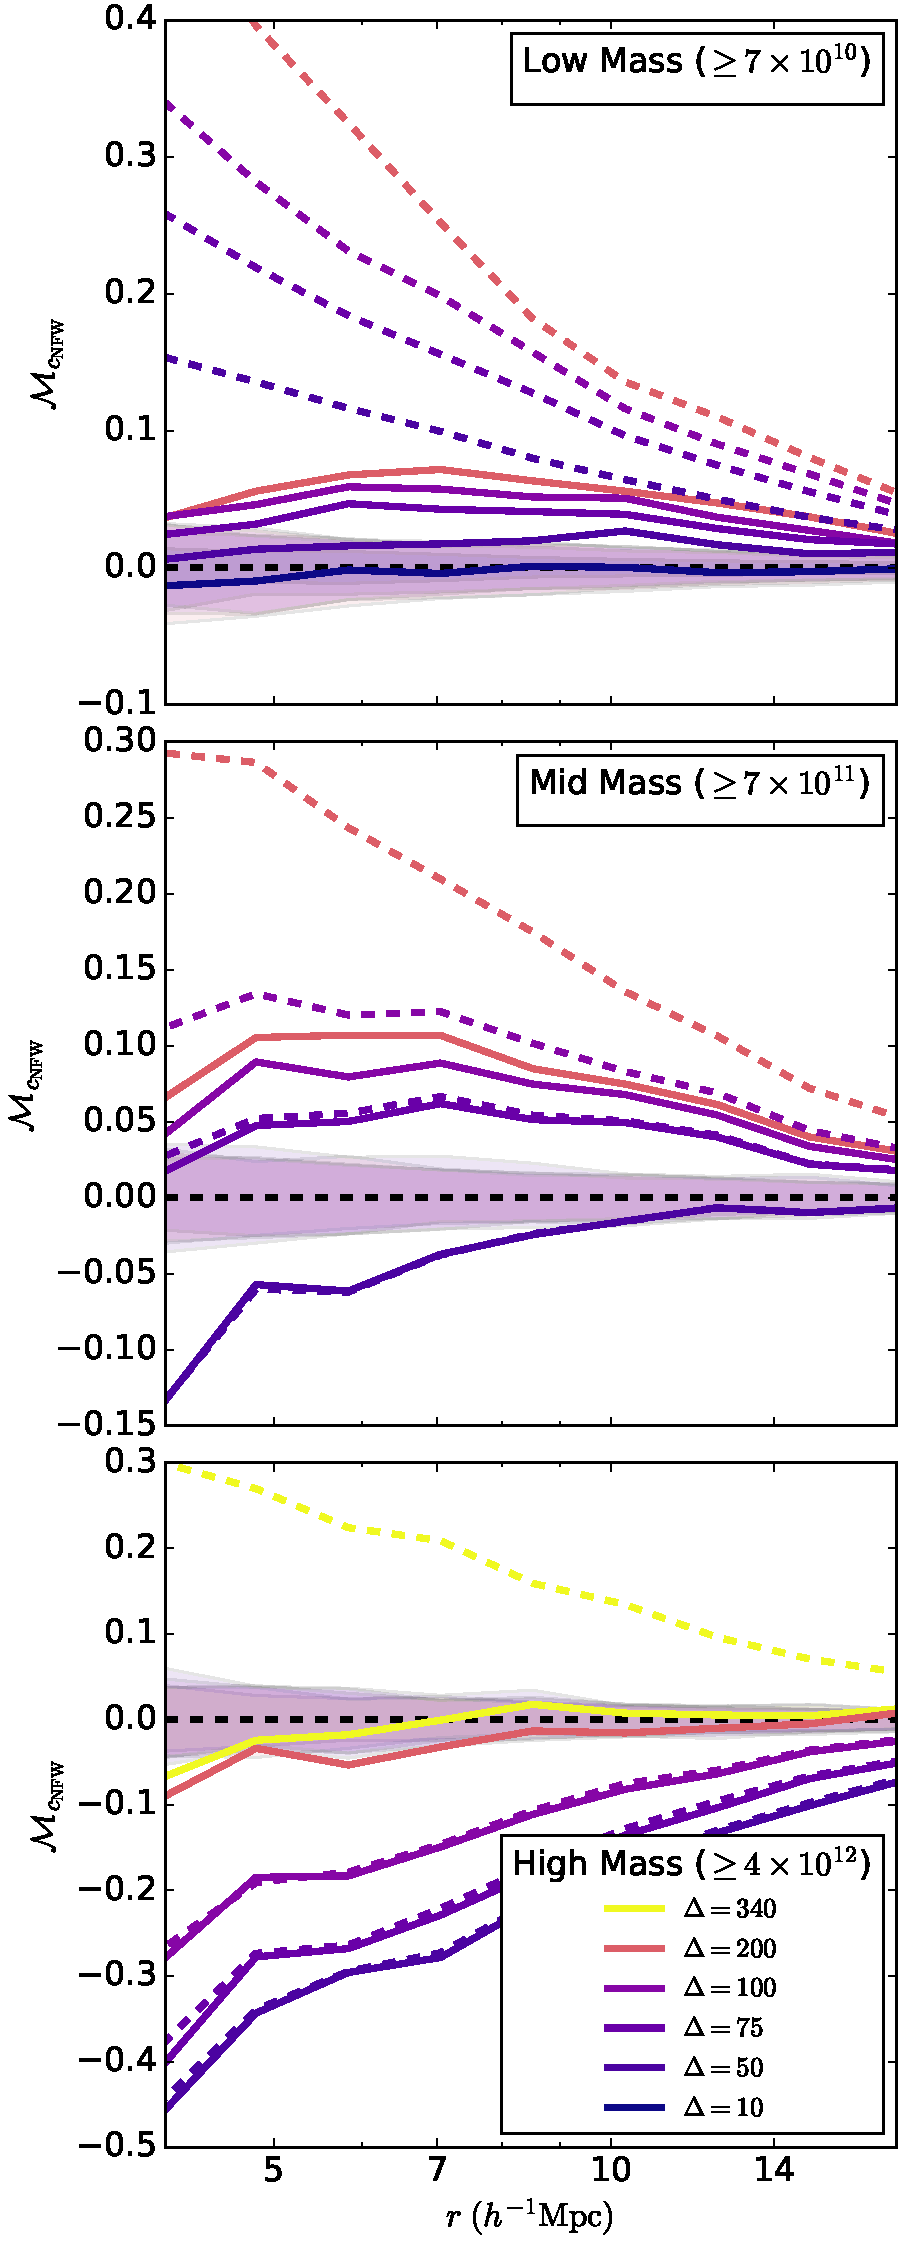
\includegraphics[width=\textwidth]{match_mcf_cNFW.pdf}
	\caption{The marked correlation function for the NFW-defined halo concentration parameter. The solid lines plot the marked correlation function using NFW-defined halo concentration as the mark, for a catalog matched against the best fit $\Delta$ shown in red. The dashed lines plot the original marked correlation function results. In each plot the lines correspond to different values of $\Delta$, with dark blue (light blue) corresponding to $\Delta = 340$ ($\Delta = 50$). The red dashed line corresponds to the overdensity chosen for matching as possibly removing assembly bias on most scales for halo concentration. The top (middle/bottom) panel shows the results for the
\simA \ (\simB /\simC) data set utilizing the low mass (mid mass/high mass) cutoffs. The shaded bands represent 2-sigma confidence regions generated by randomization of the marks. Only host halos consistent with the best-fit catalog from above are included in the analysis.\bdr{This caption describes what the figure shows, but not what it means. If I understand it correctly, this figure allows us to distinguish the different ways in which changing Delta changes assembly bias?}}
	\label{fig:hvm_mcf_cnfw}
\end{figure*}


%---------------------------------------------------------------------------------------------
\section{Discussion}
\label{section:discussion}
%---------------------------------------------------------------------------------------------

%----------------------------
\subsection{Broad Conclusions}
%----------------------------

We have studied the clustering of dark matter halos as a function of halo properties other than mass. We have confirmed that for conventional halo definitions halo clustering strength is a strong function of the  ``auxiliary properties'' that we studied, namely halo concentration (either measured through a fit to the NFW profile or assigned non-parametrically as the ratio of the maximum circular velocity to the virial velocity), halo shape, and halo spin. These findings are consistent with the now significant literature on the subject subject of halo assembly bias. \citep{peacock_smith00, wechsler_etal02,sheth_tormen04, gao_etal05, zentner_etal05, allgood_etal06, harker_etal06, wechsler_etal06, croton_etal07, zentner07, dalal_etal08, zentner_etal14, mao_etal15, sunayama_etal16}

We have explored auxiliary property dependent halo clustering as a function of halo definition, parameterized by overdensity parameter $\Delta$. This exploration was motivated, in part, to determine whether alternative halo definitions can mitigate the dependence of halo clustering on these ``auxiliary properties.'' In general, we find that these alternative halo definitions do {\em not} generally mitigate the effects of assembly bias. We are led to this conclusion for two reasons. First, no single halo definition serves to mitigate auxiliary property dependent clustering for all of the auxiliary properties that we have investigated. Indeed, modified halo definitions, with low values of $\Delta$, often lead to stronger auxiliary property dependent clustering as is the case with halo spin, for example.

Second, the halo definitions that mitigate assembly bias are strongly halo mass dependent. In the case of halo concentration, which we examine in the most detail, assembly bias is strongly mitigated for halo definitions of $\Delta \approx 20$, $\Delta \approx 40$, and $\Delta \approx 250$ for halos in our $M \geq 1.83 \times 10^{11} \hMsun$, $M \geq 7.1 \times 10^{11} \hMsun$, and $M \geq 4.06 \times 10^{12} \hMsun$ mass threshold samples respectively. Of course, this mass dependence may not be surprising given the well-known mass dependence of assembly bias. These two observations together suggest that it may well be possible to mitigate assembly bias for a single halo property (e.g., concentration) by using a mass-dependent halo definition. We discuss the particular case of concentration-dependent clustering further below.

Our work emphasizes the important dependence of halo assembly bias upon halo definition, which is not yet widely appreciated. In each of Figures \ref{fig:cc_mcf_cnfw} through \ref{fig:cc_mcf_spin}, the strength of assembly bias is a strong function of halo definition. This definition dependence is not restricted to extreme choices of the overdensity parameter $\Delta$. The difference in the strength of assembly bias between a ``virial'' halo definition, with $\Delta=340$, and a definition with $\Delta=200$ is considerable. Likewise, defining halos using an overdensity of 200 relative to the critical density, corresponding roughly to $\Delta \approx 625$ in our notation, also leads to significant, quantitative differences in the strength of assembly bias. Indeed, distinct halo definitions may even lead to assembly bias of opposite sense. For example, at fixed halo mass, higher concentration halos may be more strongly clustered by one halo definition and more weakly clustered by another. It is interesting to consider that some of the variety of results pertaining to the strength of assembly bias in the literature may be partly induced by the different halo definitions used by different authors.


%------------------------------------------------
\subsection{How Does Halo Definition Mitigate Concentration-Dependent Halo Clustering}
%------------------------------------------------

As mentioned above, our results indicate that one may mitigate auxiliary 
property dependent clustering through a mass-dependent choice of halo 
definition. It is interesting to ask why halo redefinitions may be 
helpful. In this subsection, we discuss the particular case of halo 
concentration dependent clustering in more detail in part because concentrations may be the most physically interesting property that we 
hav examined.

Halo redefinitions may mitigate concentration-dependent halo bias for at least two reasons. The physical motivation for exploring halo redefinitions is that they may identify regions with halos in a more practically useful way, incorporating objects that have been strongly affected by nonlinear evolution into a single halo and isolating them from the larger-scale environment. In such a case, halo redefinition is physically motivated and step forward. However, it is also possible that the details of measuring halo properties using these new halo definitions introduce new sources of noise into the measurements. The inherently noisier measurements then lead to reduced correlations. In this case, the reduction in correlations arises because the property of interest may be {\em less} informative about the halo itself. \bdr{After starting the paragraph saying that there are two ways, I expect a concise summary of those before going into detail. I'm not sure I got that information from the paragraph.}

For the case of halo concentration, which is the most interesting to 
follow up, noise may be introduced in numerous ways. For example, 
the NFW concentration $c_{\mathrm{NFW}}$ is determined by a fit to the 
NFW profile. Inferred values of $c_{\mathrm{NFW}}$ will depend upon 
the degree to which the density profiles of the halos follow the NFW 
functional form within some radius $R_{\Delta}$ that is different from 
traditional halo radii, such as $\sim R_{200}$. At large halocentric 
distances ($r \gtrsim R_{200}$) halo profiles are known to deviate 
from the NFW form. It may be possible to reduce assembly bias by redefinitions if one probes scales on which halos deviate from NFW in a way that is not well correlated with the interior structure of the halo (particularly the location of the NFW scale radius); however, such a reduction in assembly bias is of limited practicality because it arises from characterizing a halo by a quantity that is less informative about its interior structure. Of course, it is worth noting that the velocity-defined concentration $c_{\rm V}$ is a non-parametric measure of concentration and should be less subject to such effects. 

We can explore in more detail the degree to which the mitigation of environmental effects by halo redefinition are due to introducing noise 
that is uncorrelated with environment into the measurement of halo properties. We proceed as follows. All host halos that are found in the halo catalogs constructed from lower values of $\Delta$ (e.g., $\Delta=40$) are also present as host halos in the halo catalogs constructed with all higher values of threshold density (e.g., $\Delta=200>40$). The converse is not true because lowering $\Delta$ increases halo radii so that host halos at higher values of $\Delta$ may become subhalos at lower values of $\Delta$\footnote{Indeed, this is largely the motivation for exploring various $\Delta$!}. Therefore, we consider the clustering of only those host halos that exist in a higher $\Delta$ catalog as well as a lower $\Delta$ catalog. As a matter of clarification, an example is to consider the clustering of the subset of host halos identified within the the $\Delta=200$ catalog (and with all properties assigned to a conventional $\Delta=200$ halo), that also exist within a $\Delta=40$ catalog. Those host halos that {\em do not} exist in the $\Delta=40$ catalog are precisely those halos that have been subsumed by the larger halo radii in this case and thus been classified as subhalos. This achieves the goal of redefining halos by the lower $\Delta$ threshold ($\Delta=40$ in this example), but eliminates that fact that the properties we are studying are also defined differently in the lower $\Delta$ catalog, because we are studying their clustering as a function of the properties defined in the higher $\Delta$ ($\Delta=200$ in this example) catalog. We refer to samples constructed in this way as ``matched'' halo samples between two values of threshold overdensity $\Delta$. 


The dashed lines in Figure~\ref{fig:hvm_mcf_cnfw} show the same MCFs depicted 
in Fig.~\ref{fig:cc_mcf_cnfw}. The solid lines in Fig.~\ref{fig:hvm_mcf_cnfw} show MCFs for halo samples in ``matched'' halo catalogs in which the lower $\Delta$ is indicated in each panel (and depicted by the red, dashed lines). These lower 
values of $\Delta$ are chosen to effectively remove assembly bias at large scales based on the results in Fig.~\ref{fig:cc_mcf_cnfw}, 
$\Delta=20$ for the `Low Mass' cut, 
$\Delta=40$ for the `Mid Mass' cut, 
and $\Delta=250$ for the `High Mass' cut. 

In comparing a pair of dashed and solid lines at the same $\Delta$ threshold in Fig.~\ref{fig:hvm_mcf_cnfw}, one is comparing the MCF of all halos at that $\Delta$ threshold, to the MCF of only those halos identified in the lower threshold samples. The difference between a pair of solid and dashed lines at fixed $\Delta$ is caused entirely by the exclusion of some halos from the lower $\Delta$ catalog due to a change in halo definition. Notice that the solid lines exhibit greatly reduced concentration-dependent clustering. Selecting particular halos as hosts eliminates a large contribution to concentration-dependent clustering. Fig.~\ref{fig:hvm_mcf_cV} displays analogous results for the velocity-defined concentration parameter $c_{\rm V}$. These results suggest that much of concentration-dependent clustering is driven by the interactions of nearby halos. They also suggest that subsuming larger regions into halo definitions to accommodate these interactions may be well motivated and practically useful in the context of halo occupation models. It may even be possible to optimize halo definitions for specific applications. 

In each panel in Fig.~\ref{fig:hvm_mcf_cnfw}, there is some modest residual assembly bias displayed by the solid lines; the solid lines are not all consistent with zero. This suggests that redefining halos with larger radii (smaller $\Delta$) may, in part, reduce assembly bias through the introduction of noise in the concentration measurement, rendering it less informative about the interior structure of the halo. Nonetheless, this residual assembly bias is generally modest compared with the concentration-dependent clustering of halos defined with more traditional values of overdensity threshold.

%-------------------------------------------
\begin{figure*}
	\centering
	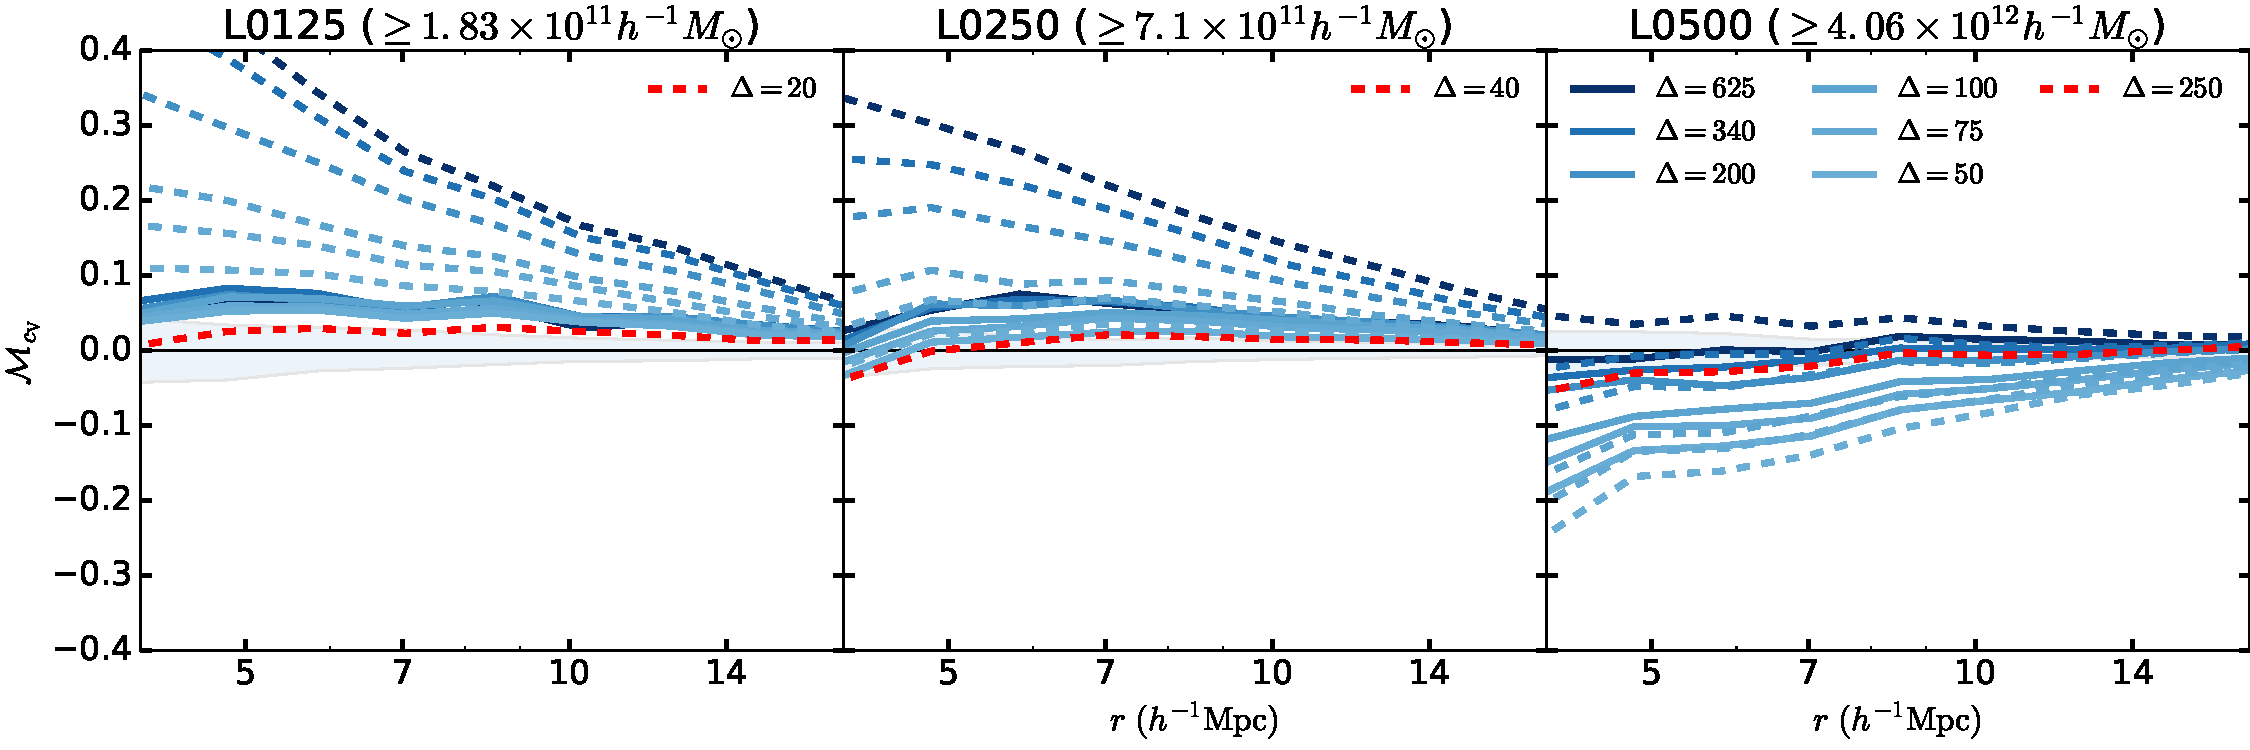
\includegraphics[width=\textwidth]{match_mcf_cV.pdf}
	\caption{As Fig.~\ref{fig:hvm_mcf_cnfw}, with the mark defined as velocity ratio defined concentration. \yao{seems repeating with Fig.~\ref{fig:hvm_mcf_cnfw}}}
	\label{fig:hvm_mcf_cV}
\end{figure*}
%-----------------------------------------------

%---- Splashback Comparison
\subsection{Halo Definitions and the Splashback Radius}

Our study is reminscent of, and indeed motivated by, much of the recent work on halo splashback radii \citep{more_etal15}. \arz{Cite Phil Mansfield's paper here as well.} Briefly, the splashback radius of a halo is intended to be the halo-centric distance that characterizes the orbital apocenters of accreted halo material. It is, therfore, a well motivated criterion for separating the halo region, within which halo interactions are clearly important, from larger scales, where halo interactions may be less important. Our perspective is to generalize this idea by identifying the importance of interactions by investigating the environment dependence of halo properties themselves (e.g., halo concentrations). Consequently, it is interesting to compare our results with halo splashback radii. 

In Figure~\ref{fig:splashback_compare}, we show a first, broad comparison of our work with halo splashback radii. The blue points in Fig.~\ref{fig:splashback_compare} show the radii (in units of the traditional $R_{200}$ halo radius) of halos selected at each of the $\Delta$ thresholds that minimize concentration dependent halo clustering as a function of halo mass $M_{200}$. As we have already remarked, our work suggests that halo definition must be a rapidly varying function of halo mass in order to mitigate assembly bias. The red points depict the mean halo splashback radii of halos of fixed mass as a function of $M_{200}$ \citep[from][]{more_etal15}. Clearly, our results suggest that identification of halos using splashback radii alone will not greatly mitigate assembly bias. 

%-------------- splashback comparison --
\begin{figure}
	\centering
	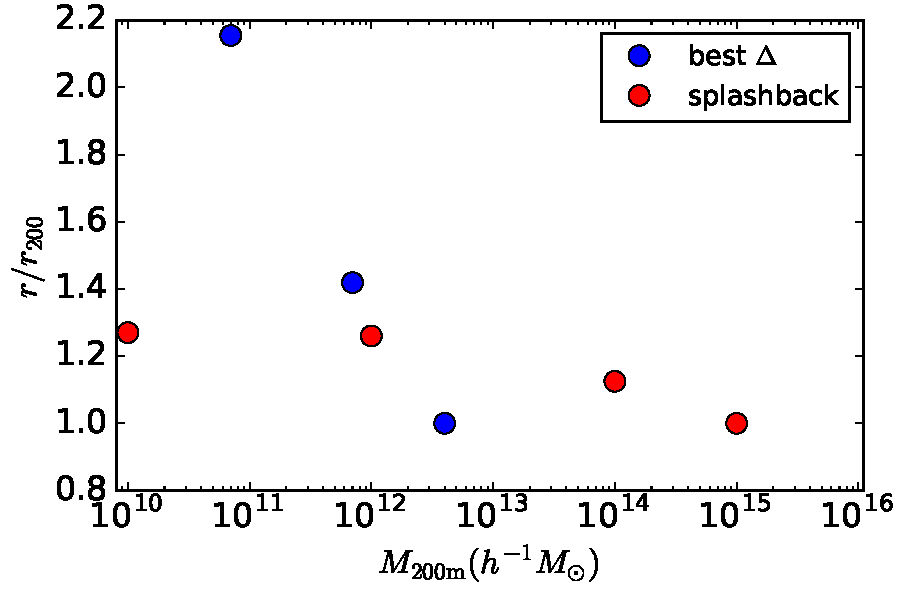
\includegraphics[width=\columnwidth]{test_splashback.pdf}
	\caption{A comparison of the average ratio between $r_{200}$ and the splashback radius as determined by
	 \citet{diemer_etal17} (red line) to the average ratio between $r_{200}$ and the halo radius determined as our
	  best fit for removal of assembly bias as discussed above (blue circles). Note that the halo mass chosen for
	  the blue points is determined by the mass cutoff in the simulation analysis, as the smallest (and most
	  numerous) halos dominate the calculation. \yao{maybe change the red dots (theory) to a red line (but keep blue dots as dots)?}\bdr{I agree with Yao, the red should definitely be a line.The More15 result was derived in a very crude way, could we please replace it with the new Diemer17 fit? This new function is redshift-dependent, adding a new dimension to the problem. But we could also show the z=0 line for simplicity. Also, what exactly are the blue circles? The mean of all the Deltas you find for c, spin etc? I might be better to show these Deltas as separate points so that the reader gets a summary of the results, and can put a crude error bar on the Deltas.}}
	\label{fig:splashback_compare}
\end{figure}
%---------------------------------------


%---Concentration-Dependent Halo Bias
\subsection{Concentration Dependent Halo Bias as a function of Halo Definition}

Concentration-dependent halo clustering is already been found to be halo mass dependent and our work confirms this mass dependence. As we noted above, our work places emphasis on the fact that concentration-dependent halo clustering (and auxiliary property dependent halo clustering) is strongly dependent upon halo definition. Figure~\ref{fig:biascompare} summarizes both of these aspects of concentration-dependent clustering. Fig.~\ref{fig:biascompare} shows the {\em relative} bias of high concentration halos compared to all halos defined as: 
\beq
b^2(r) = \xi_{c_\mathrm{NFW},80\%} / \xi_{\mathrm{all}},
\eeq
where $\xi_{c_\mathrm{NFW},80\%}$ designates the clustering of halos in the $80^{\mathrm{th}}$ percentile of halo concentration at fixed mass (that is, the halos with the $20\%$ highest concentrations). To summarize clustering 
strength with a single relative bias, we computed pair counts within a wide bin of separations from $5-10\, \hMpc$. We estimated the errors on the relative bias by recomputing $\xi_{\mathrm{all}}$ using randomly-selected subsamples of equal number to the subsample used to compute $\xi_{c_{\mathrm{NFW}},80\%}$, that is, using one fifth of all halos. 
The error bars show the $68\%$ range, centered on the median, about which the values of $b^2(r)$ lie. 

Both the mass dependence of concentration-dependent halo clustering and its depdence upon halo definition are evident in the figure. This suggests that a great deal of care must be taken in comparing the work of groups that use distinct halo definitions. Beyond that, it also suggests that in order to interpret high-precision clustering data it is imperative to develop notions of halos that are governed by practical criteria. These practical criteria may be a more useful separation between interacting and non-interacting halos (as we have attempted here). Another practical consideration may be defining halos such that we suspect, on physical grounds, that their properties should be correlated with the properties of the galaxies they host. 

%----------------------------------------
\begin{figure*}
	\centering
	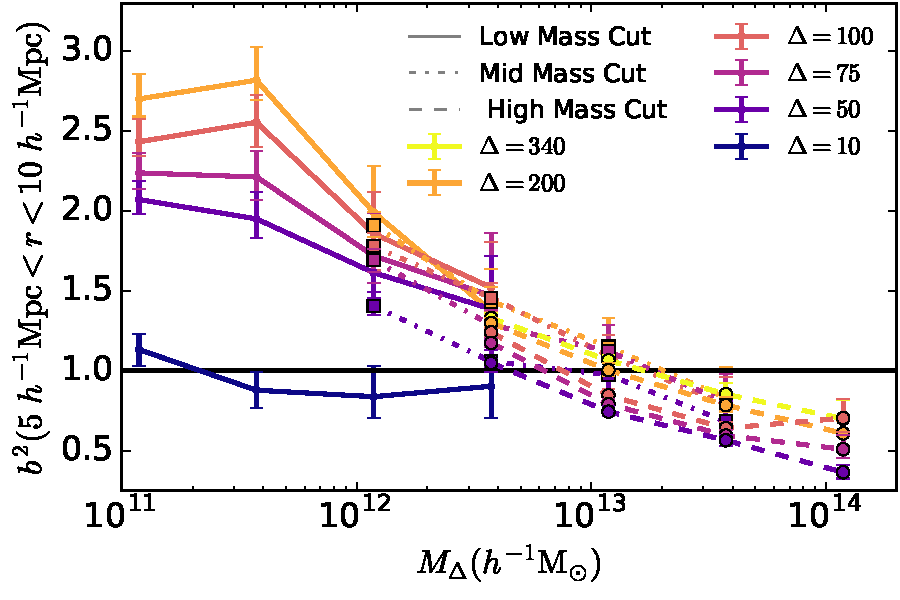
\includegraphics[width=\textwidth]{biasplot.pdf}
	\caption{
    \arz{Can you put a $\Delta=20$ line on this plot? Can you make this plot with a square aspect ratio?}\asv{I'll see about getting square aspect ratio in the next major pass. $\Delta = 20$ would take more time as I would need to do some L0500 reruns and we are currently grinding out $\Delta = 625$.}
	The bias of the 20\% highest concentration sample to the full sample, plotted against halo mass measured at the halo radius. The halo mass binning is defined in full detail in the text. Halo definitions descend from the largest definition to lowest definition, from dark to light in color. The dark blue (light blue) line uses a halo definition drawn from $\Delta = 340$ ($\Delta = 50$). The solid (dot-dashed, dashsed) lines use host halos from the \simA (\simB,\simC) catalogs. The
	error bars encompass 68\% of measurements using two hundred subsamples
	of the mark of the same size as the biased sample. The solid black line
	shows where there is no detected assembly bias driven by NFW-defined halo concentration.}
	\label{fig:biascompare}
\end{figure*}
%--------------------------------------------


%----------------------
\section[]{Conclusions}
\label{section:conclusions}
%----------------------
We have explored how halo redefinition can be applied to mitigate assembly bias on auxiliary halo properties. We have tested this method across a wide range of halo masses taking advantage of the \citet{diemer_kravtsov15} simulation suite. Using both correlation functions and marked correlation functions (MCFs), we test how auxiliary halo properties drive halo assembly bias. We draw attention to the following conclusions:
\begin{itemize}
    \item The auxiliary property of halo concentration \bdr{awkward phrasing... I'd just say concentration} shows the most promise for assembly bias mitigation. Halo redefinition reduces the impact of halo assembly bias. Figure \ref{fig:hvm_mcf_cnfw} strongly suggests that our method accomplishes this mitigation through the exclusion of halos from the catalog \bdr{...by making them subhalos}. However, there is no mass-independent definition to this halo redefinition: a definition of $\Delta=20$ that mitigates assembly bias at low masses ($M_{200} > 1.83\times10^{11}\hMsun$) in fact induces assembly bias of opposite sign (e.g., clustered halos have preferentially smaller concentrations) at high masses ($M_{200} > 4.06\times10^{12}\hMsun$).
    \item The auxiliary property of halo shape requires an extreme halo definition to remove assembly bias; we consider halo redefinition infeasible for mitigating shape-driven assembly bias. This may be suggestive of environmental effects impacting halo shape measurements on scales significantly larger than $\Rvir$.
    \item The auxiliary property of halo spin demonstrates increased assembly bias with halo mass. Assembly bias is mitigated for $\Delta \sim 340$ for the lowest masses ($M_{200} > 1.83\times10^{11}\hMsun$), while larger values of $\Delta$ must be explored for the highest masses. The fact that spin-driven assembly bias increases as we increase $\Rdel$ is suggestive of the impact of large scale structure upon this measurement.
    \item We note that though similarities exist between our methodology and recent studies \citep{more_etal15} focusing on implementation of a ``splashback radius'', there is no clear connection between our best fit values of $\Delta$ and the splashback radius at this time. This remains an exploration for future work.
    \item We show that the halo bias ratio for the $80^{\mathrm{th}}$ percentile cut on concentration is dependent on both halo definition and halo mass. Comparison between different works in the literature may be difficult without taking into account the impact of this.
\end{itemize}

The results, while not perfect in mitigating assembly bias, are encouraging. They show a potential for being able to mitigate the impact of assembly bias through a change of halo definition. This may lead us to better halo models that allow for easier comparison to observables and a better understanding of complicated problems such as galaxy assembly bias. However, we almost certainly will require more information than a single value of the overdensity parameter. Future work will investigate how we may improve this methodology. It is possible that including additional information on a halo-by-halo basis, such as the method of the splashback radius promises, might be the change in halo size that is most promising.

There are several clear paths of follow-up to gain a better understanding of how halo definition impacts both the halo model and observables. While we cover a large range of halo masses in this study, we may be able to extend the explored mass range through the use of larger simulation volumes and simulations with higher mass resolution. Further, we do not explore how this relationship may evolve with redshift or cosmology. We hope to extend our framework to exploring these possibilities in future work, as the implications for deviations from the $z=0$ relation for assembly bias is important in both observational and simulation work.

\section*{Acknowledgments}

We are grateful to many people. Our calculations are carried out utilizing the
{\tt numpy} \citep{numpy}, {\tt astropy} \citep{astropy}, {\tt matplotlib} 
\citep{matplotlib}, and {\tt halotools} \citep{halotools} packages in Python.

\bibliographystyle{mnras}
\bibliography{master}

\section*{Appendix}
\label{section:appendix_massres}
\asv{This appendix is probably entirely extraneous at this point. I am not sure if it should be removed or if we want to reword it with a different set of plots. Originally, this showed the higher mass cuts extrapolated down to the lower size simulation boxes, which resulted in the same impact with more noise. I could regenerate those plots (they were in a pre-{\tt halotools} version of the code, but it shouldn't take too long with the new ranked version to remake them), or we could leave the figures out. I am inclined to say the paper is crowded with enough figures as it is though.}
One natural question that might arise in the analysis of this work is the nature of the resulting assembly bias
trends. Our focus in the main sections of this paper is on the nature of the assembly bias changing as a function
of the mass cut chosen. Our conclusions include the fact that there is a strong mass dependence on halo assembly
bias that must be accounted for separately depending on the halos of interest in a study. However, while the
existence of this trend is clear within our analysis, the determination that this is solely due to the masses of
the halos included in our calculation is less clear upon closer inspection. One possibility that might be
particularly concerning is the potential that the different simulations have created halos that have
fundamentally different clustering and this is leading to the result that we are interpreting as a mass
dependence on assembly bias. Thankfully, though our statistics become less meaningful to carry out this
calculation, we can carry out a comparison using the same mass cut across two of our simulations, knowing that
these will only contain well resolved halos.

While not addressed directly, Figure~\ref{fig:hvl_cfcompare} through Figure~\ref{fig:hvl_mcf_nsat} \yao{where are these figures?}\asv{These figures evolved into the ones further back when we decided to focus on the mass resolution aspects rather than a single common solution.} contain a
demonstration of the result that we are seeking in the left column of panels. The lower left panels show various
marks of interest for \simB \ using the ``mid mass'' cut on the data set. In comparison, the upper left panel
contains the same marks of interest for the \simA \ using the same mass cut. In the latter, there are fewer halos
in this mass cut range, as a result of the smaller simulation box size. However, we note that despite the
additional noise in the data set, the behavior of the assembly bias measurement is nearly identical within
tolerances accounting for differences between simulations and noise. This motivates our conclusion that the
driver behind the behavior is the mass cut of the data sets rather than the resolution of the simulation.

\label{lastpage}

\end{document}
